% Final Course Project -- Survival Analysis and Machine Learning, Spring 2026
% Oded Katz (211862693), Diana Morgan (336472261)
\documentclass[11pt,a4paper]{article}

\usepackage[T1]{fontenc}
\usepackage[utf8]{inputenc}
\usepackage[margin=2.5cm]{geometry}
\usepackage{mathptmx}                 % Times New Roman-like text and math
\usepackage{setspace}
\usepackage{amsmath}
\usepackage{graphicx}
\usepackage{booktabs}
\usepackage{float}
\usepackage[font=small,labelfont=bf,justification=justified,labelsep=period]{caption}
\usepackage{xcolor}
\definecolor{linknavy}{HTML}{1A4E8A}
\usepackage{hyperref}
\hypersetup{colorlinks=true, linkcolor=linknavy, citecolor=linknavy, urlcolor=linknavy}

% make the whole phrase clickable, not just the numeral
\newcommand{\tabref}[1]{\hyperref[#1]{Table~\ref*{#1}}}
\newcommand{\figref}[1]{\hyperref[#1]{Figure~\ref*{#1}}}

\setstretch{1.15}
\setlength{\parskip}{0.5em}
\setlength{\parindent}{0pt}
% figs/ resolves when compiling inside this folder; latex/figs/ when Overleaf
% compiles from the project root with latex/Report.tex as the main file
\graphicspath{{figs/}{latex/figs/}}

% shorthand for the change in BUN over the admission
\newcommand{\dbun}{$\Delta$BUN}

\title{\vspace{-1.5cm}\bfseries Predicting One-Year Survival After Hospital Discharge:
A Comparison of Cox Regression, Random Survival Forests, DeepSurv and Cox-Time}
\author{Oded Katz (211862693) \quad$\cdot$\quad Diana Morgan (336472261)}
\date{Survival Analysis and Machine Learning --- Final Course Project\\
Data and Decision Sciences, Technion --- Spring 2026}

\begin{document}
\maketitle

%======================================================================
\section{Introduction}

This project builds on Project Assignments 1 and 2 using synthetic dataset 2. PA1 provided an exploratory analysis of the covariates, missingness, survival outcome, censoring, and Kaplan--Meier curves. PA2 then developed a Cox proportional hazards model, tested whether the change in BUN during admission added information beyond the discharge level, assessed the proportional hazards assumption, and compared the Cox model with a log-normal AFT model. Both models were fitted to the full dataset and evaluated using in-sample summaries. Their performance for previously unseen patients therefore remained unknown.

The present analysis focuses on out-of-sample prediction. The data are split into 80\% training and 20\% test sets. The Cox model from PA2 is refitted on the training data and compared with three more flexible approaches: a random survival forest (RSF), DeepSurv, and Cox-Time. These models relax different assumptions of the Cox model, including linearity on the log-hazard scale, additivity of covariate effects, and constant hazard ratios over time. The comparison therefore addresses two questions: whether additional flexibility improves prediction, and which Cox model assumptions, if any, appear to limit performance.


%======================================================================
\section{Data and preprocessing}

Synthetic dataset 2 contains 3,961 patients admitted with acute decompensated heart failure who were discharged alive. Each patient is described by 25 covariates, including demographics, nine comorbidity indicators, admission and discharge laboratory measurements, and length of stay (\tabref{tab:covariates}).

The event of interest is death from any cause, with survival time measured in months from discharge. Follow-up ends administratively at 36 months, so patients who remain alive at that point are right-censored. Of the 2,282 censored patients, 1,473 reach the 36-month cutoff, while 809 are censored earlier, with a median censoring time of 16.5 months. Censoring is assumed to be independent of survival time conditional on the covariates. Median follow-up is 25.6 months (IQR 8.8--36.0). By the one-year prediction horizon used throughout the analysis, 947 deaths have occurred and 328 patients have been censored (\tabref{tab:cohort}).

Following PA1, missing values in continuous covariates were imputed using the median; no categorical covariates contained missing values. Following PA2, the nine comorbidity indicators were summarized as comorbidity burden and grouped into 0--1 (reference), 2--3, and 4+ comorbidities. In addition, \dbun{} $=$ BUN at discharge $-$ BUN on admission was constructed.

The cohort is predominantly older and highly comorbid. Median age is 76 years, 46.5\% are women, 86.6\% have hypertension, and 62.7\% have ischaemic heart disease. Median BUN increases from 25,mg/dL on admission to 28,mg/dL at discharge.


%======================================================================
\section{Brief recap of the previous analyses}

\subsection{Project Assignment 1}

The overall Kaplan--Meier curve (\figref{fig:km-overall}) declines to approximately 0.53 by 36 months, with the steepest drop occurring during the first few months. At one year, roughly three quarters of the cohort remain alive.

Sex and diabetes show little separation in survival (\figref{fig:km-sex-dm}). One-year survival is 0.770 versus 0.733 between the two sex groups, and 0.740 versus 0.764 for patients with and without diabetes. In contrast, age and discharge BUN show clear differences when split at their medians (\figref{fig:km-age-bun}). One-year survival is 0.661 for patients older than 76 years compared with 0.844 for younger patients, and 0.676 for discharge BUN above 28,mg/dL compared with 0.810 below this threshold. The confidence bands remain clearly separated over follow-up.

\subsection{Project Assignment 2}

PA2 selected a Cox proportional hazards model including sex, age, comorbidity burden, length of stay, discharge BUN, discharge creatinine and GFR, BNP, white blood cells, sodium, RDW, platelets, bilirubin, potassium, and \dbun{} (\tabref{tab:pa2cox}). The model achieved an in-sample concordance of 0.694.

Nine model terms were statistically significant. Higher age, discharge BUN, RDW, and BNP were associated with increased hazard, with hazard ratios of 1.044 per year, 1.021 per mg/dL, 1.120 per RDW unit, and 1.0002 per pg/mL, respectively. Sodium, potassium, and \dbun{} had hazard ratios below 1. Sex, comorbidity burden, white blood cells, discharge creatinine, discharge GFR, and platelets were not significant.

\dbun{} added information beyond discharge BUN alone. A likelihood-ratio test comparing the full model with a model excluding \dbun{} gave $\chi^2 = 27.63$ on 1 degree of freedom, with $p = 1.5 \times 10^{-7}$. It was therefore retained in all subsequent models. A Schoenfeld residual test using a rank transformation of time identified two of sixteen terms as potentially violating proportional hazards: discharge BUN ($p=0.036$) and length of stay ($p=0.048$). Because both results were marginal, PA2 treated the violations as mild.

A log-normal AFT model fitted to the same covariates produced effects in the same direction as the Cox model. One-year predictions from the two models (\figref{fig:cox-aft}) are nearly identical across age, show somewhat greater separation for RDW, and differ most for discharge BUN. For BUN, the AFT prediction decreases more rapidly in the middle of the observed range before crossing above the Cox prediction in the upper tail. The original figure extends BUN to its observed maximum of 236,mg/dL, although 75% of patients have values below 39,mg/dL. For this reason, percentile-based grids are used from Section~6.2 onward.


%======================================================================
\section{Research questions}

PA1 closed with three questions:

\begin{quote}\itshape
RQ1 (PA1). Does the difference between BUN on admission and on discharge have a significant
effect on the survival outcome?
\end{quote}

\begin{quote}\itshape
RQ2 (PA1). Are there covariate interactions with a significant effect on the survival
outcome?
\end{quote}

\begin{quote}\itshape
RQ3 (PA1). How accurately can survival be predicted at hospital discharge?
\end{quote}

The first is answered by PA2's \dbun{} test. The second was never addressed, and as phrased
it does not say which interactions to look for; testing all 105 covariate pairs would
produce significant results by chance alone. The third was not addressed either, since both
assignments reported in-sample summaries. The final research questions are the following.

\begin{quote}\itshape
RQ1. How accurately can one-year survival be predicted from the information available at
discharge, and do the more flexible models predict better than the Cox model?
\end{quote}

Sections 5.1--5.4 fit the four models on the training set and Section~6.4 compares them on
the test set.

\begin{quote}\itshape
RQ2. Where the more flexible models differ from the Cox model, which of the Cox model's
assumptions is responsible?
\end{quote}

DeepSurv relaxes linearity and additivity but keeps hazards proportional; Cox-Time also
lets the risk score depend on time; the forest assumes none of the three. Section~3.2 gives
a reason to ask, as proportional hazards came out borderline for discharge BUN and length
of stay.

\begin{quote}\itshape
RQ3. Do the two interactions specified below improve on the additive Cox model?
\end{quote}

Two terms fixed in advance rather than a search over all pairs. \dbun{} with discharge BUN,
since the change and the level are tied by construction and the same change plausibly means
different things depending on the level reached, which an additive model cannot express; and
age with discharge BUN, the two strongest predictors in \tabref{tab:pa2cox}. Each is added as a single
term to the refitted Cox model and tested by a likelihood-ratio test in Section~6.7, against
a Bonferroni-corrected threshold of 0.025. All analyses use comorbidity burden rather than
the individual indicators, which no question requires.

%======================================================================
\section{Methods}

\subsection{Train--test split}

The data were split once, 80/20, with the seed fixed at 42. That seed is set once and
governs every random step: the split, the cross-validation folds, the forest's bootstrap
samples and feature sampling, and both networks' initialisation and batching. The split is
stratified by the event indicator, so both sets carry the same event rate (\tabref{tab:split}): 3,168
training patients with 1,343 events and 793 test patients with 336. The test set is
untouched until Section~6.4 and used once. Its 199 one-year deaths bound how finely it can
distinguish between models.

\subsection{The Cox model and one-year prediction}

The model was refitted on the training patients with the same formula. Because lifelines
centres the covariates,
\[
  \hat S(12 \mid X) = \hat S_0(12)^{\exp\left((X - \bar X)^{\top} \hat\beta\right)},
\]
with $\hat S_0$ the Breslow baseline and $\bar X$ the training covariate means;
$\hat S_0(12) = 0.790$ is therefore the prediction at those means, not at zero.

Prediction plots hold all covariates but one at representative training values: medians for
continuous covariates and the most common level for comorbidity burden. Sex is the only
binary covariate and its median coincides with its most common category, so medians
throughout give the representative patient --- a man of 76 with two or three comorbidities,
discharge BUN 28\,mg/dL, RDW 15.3\% and a five-day stay --- whose predicted one-year
survival is 0.821. Grids run from the 1st to the 99th training percentile: discharge BUN
reaches 199.7\,mg/dL while its upper quartile is 38, so a full-range axis would be mostly
empty. The same grids and representative patient are reused in Section~6.3.

\subsection{The three additional models}

All three use the same training patients and the same sixteen design terms as the refitted
Cox model --- fourteen continuous covariates plus two comorbidity burden dummies --- so
that differences come from the model and not from the inputs.

\textbf{Random survival forest.} 500 trees on bootstrap samples of the training data. Each
node splits on the covariate and cut point maximising the log-rank statistic between the two
children, each terminal node carries the Nelson--Aalen cumulative hazard of its training
patients, and a patient's survival curve is the average over trees. Tuned: minimum leaf size
over 5, 15, 30 and 50, and features per split over 4, 8 and 16. Leaf size sets how many
patients stand behind each terminal estimate --- at a 42\% event rate a leaf of five holds
about two deaths --- while restricting features decorrelates the trees but risks leaving the
strong covariates unavailable at a split. Fixed: 500 trees, minimum split size twice the
leaf size, unbounded depth.

\textbf{DeepSurv.} Keeps the Cox partial likelihood and replaces $X^{\top}\beta$ with a
network $g(X)$, so $\hat S(t \mid X) = \hat S_0(t)^{\exp(g(X))}$ with $\hat S_0$ the Breslow
estimator. Hazards stay proportional, since $\exp(g(x_1) - g(x_2))$ does not involve $t$;
what the network adds is a risk score free to bend with each covariate and to let covariates
modify one another. Tuned: hidden layers over [16], [32, 32] and [64, 64]; dropout 0.1 and
0.4; learning rate 0.01 and 0.001. A single layer of sixteen units is close to the Cox model
and serves as a floor. Fixed: Adam, batch size 256, at most 512 epochs, early stopping after
ten epochs with the best weights restored, no output bias, standardised covariates.

\textbf{Cox-Time.} Drops proportional hazards: the risk score becomes $g(t, X)$, so the
hazard ratio between two patients can change over follow-up, and
$\hat S(t \mid X) = \exp(-\hat H(t \mid X))$ with $\hat H$ accumulating the baseline hazard
weighted by $\exp(g(t, X))$. The full partial likelihood would need the network at every
event time for everyone still at risk, so training uses case--control sampling with one
control per event. The grid, fixed settings and trainer are otherwise DeepSurv's, so the
difference between the two networks reflects the proportional hazards assumption rather than
unequal tuning; the early-stopping data are repeated ten times, since a sampled loss on one
copy is too noisy to stop on.

\subsection{Hyperparameter selection}

Hyperparameters were chosen by 5-fold cross-validation inside the training set, with the
folds drawn once and reused for all three models, and each configuration scored by the
integrated Brier score (IBS) over the first year so that tuning and evaluation target the
same quantity. Cross-validation was used rather than a single validation block because only
about a fifth of the cohort dies within the year, so one split would mostly rank noise.
Since nearby configurations differ by less than the fold-to-fold noise, a one-standard-error
rule keeps the simplest configuration within one SE of the best --- larger leaves for the
forest, fewer hidden units and then higher dropout for the networks --- refitted on all
training patients. Epochs were not tuned: 20\% of each fold's fitting data was held out for
early stopping, and the final networks trained on all training patients for the average
best-epoch count.

\tabref{tab:hyper} gives the selections. Both networks took the smallest architecture on offer with the
higher dropout rate, and the forest the largest leaf size and most restrictive feature
sampling: every search moved to the least flexible end of its grid, which anticipates the
test-set result. All four cross-validated scores lie within 0.0020 of one another, inside
the standard errors of about 0.003.

\subsection{Evaluation measures}

$\hat S(12 \mid X)$ is read off each predicted curve and the one-year risk is
$r = 1 - \hat S(12 \mid X)$. Discrimination is Uno's time-dependent C-index at
$\tau = 12$ months on the predicted risks, with censoring weights estimated on the training
data. For calibration, test patients are split into deciles of predicted one-year survival
and each decile's observed survival is its Kaplan--Meier estimate at 12 months rather than a
raw proportion, since some patients in every decile are censored earlier; the deciles are
summarised by the size-weighted mean absolute gap. Accuracy is the integrated Brier score
\[
  \mathrm{IBS} = \frac{1}{12}\int_{0}^{12} \widehat{BS}(t)\,dt
\]
over the IPCW Brier score, approximated by the trapezoidal rule on months 1 to 12 together
with $\widehat{BS}(0) = 0$, which is exact since every patient is alive at discharge and
every model predicts $S(0) = 1$.



%======================================================================
\section{Results}

\subsection{The refitted Cox model and its assumptions}

\tabref{tab:coxtrain} refits the PA2 model on the training patients. The estimates are stable: no hazard
ratio moves by more than 2.2\%, every full-data estimate falls inside the training
confidence interval, and concordance is 0.699 against 0.694. Bilirubin and potassium lose
significance (0.037 to 0.126 and 0.038 to 0.078) but their hazard ratios barely move (1.121
to 1.099 and 0.914 to 0.920); the intervals widened on 20\% less data, and both terms were
marginal already. The seven remaining significant terms are essentially unchanged, so PA2's
conclusions hold.

\dbun{} needs one clarification, since a hazard ratio below 1 reads as if a rise in BUN
during the stay were protective. With the discharge level also in the model, \dbun{}'s
coefficient is minus the effect of the admission level at a fixed discharge level: 0.990 per
mg/dL of rise says the same as 1.010 per mg/dL of admission BUN. Of two patients leaving
with the same BUN, the one who started higher does worse.

The Schoenfeld test gives a different answer on the training data (\tabref{tab:ph}). Discharge BUN
and length of stay rise to 0.116 and 0.137, while both comorbidity burden levels and
bilirubin fall below 0.05; no covariate is flagged in both fits. Since the training set is
four fifths of the cohort, a genuinely time-varying hazard ratio would still show up in the
subset, so flags that swap are noise --- the smallest $p$-value in either fit is 0.021,
unremarkable among sixteen tests. The residual smoothers are flat throughout (\figref{fig:schoenfeld}).
Proportional hazards is an adequate approximation and the hazard ratios describe average
effects over follow-up.

\subsection{One-year prediction from the refitted Cox model}

\figref{fig:cox-oneyear} and \tabref{tab:coxpred} give predicted one-year survival against age, RDW and discharge BUN.
Which covariate matters most depends on the range. Across the plotted grid discharge BUN
moves the prediction furthest, from 0.876 at 11\,mg/dL to 0.298 at 105, then age (0.962 to
0.641) and RDW (0.864 to 0.659). Over the interquartile range the order reverses: age 0.11,
discharge BUN 0.06, RDW 0.03. Age therefore separates predictions most for a typical
patient, while discharge BUN dominates the grid because of its long right tail and matters
most for the minority discharged high. All three curves decline monotonically and flatten,
which is a property of the linear predictor rather than a finding, and is the shape the next
section tests.

\subsection{Do the flexible models see the covariates differently? (RQ2)}

\figref{fig:model-curves} overlays all four models on the grids of Section~6.2 and \tabref{tab:modelcurves} quantifies them.
Over the interquartile range they agree: age moves predicted one-year survival by 0.10 to
0.12, discharge BUN by 0.03 to 0.08 and RDW by 0.03 to 0.06, and all four put age first.
Only the forest reorders the other two, ranking RDW above discharge BUN.

They part company in the tails. Across the plotted BUN range Cox falls to 0.298, Cox-Time to
0.389, DeepSurv to 0.465 and the forest to 0.719. Cox extrapolates its log-hazard slope
wherever the grid goes; DeepSurv follows it to about 40\,mg/dL and then bends upwards, while
Cox-Time runs a little below it from 40 to about 85\,mg/dL before crossing back above; the
forest flattens above about 75\,mg/dL, where only 141 of the 3,168 training patients sit and
a leaf of 50 leaves no split to make. That plateau is the forest running out of data, not
evidence that risk stops rising. RDW repeats the pattern mildly and age agrees best,
separating only past 85 years. So the flexible models find no non-linearity that the Cox
model misses where patients actually are; their disagreement is confined to the sparse
tails, and at the far end of every grid all three finish above the linear extrapolation.

\subsection{Test-set model comparison (RQ1)}

The 793 test patients are used here for the first time. Mean predicted one-year survival is
nearly identical across models (0.748, 0.751, 0.744 and 0.744 for Cox, the forest, DeepSurv
and Cox-Time) but the spread is not: the forest has standard deviation 0.118 and never
predicts below 0.441, while Cox has 0.161 and sends two patients essentially to zero ---
those with discharge BUN of 137 and 236\,mg/dL, the second beyond the training maximum of
199.7. DeepSurv reaches 0.002 at its own minimum and Cox-Time stops at 0.106. These are the
tails of \figref{fig:model-curves} from the other side: the forest cannot leave the
range its leaves cover, and Cox extrapolates without limit.

\setcounter{table}{9}   % this inline table is Table 10; back matter resumes at 1
\begin{table}[H]
\centering
\caption{Test-set performance: Uno's C-index at $\tau = 12$ months, the
integrated Brier score over the first year, and the size-weighted mean absolute difference
between predicted and observed one-year survival across the ten calibration deciles. Higher
is better for the C-index, lower for the other two.}
\label{tab:testperf}
\vspace{0.3em}
\small
\begin{tabular}{lccc}
\toprule
Model & Uno's C ($\tau = 12$) & IBS (0--12 months) & Mean $|$observed $-$ predicted$|$ \\
\midrule
Cox      & 0.6959 & 0.1150 & 0.0367 \\
RSF      & 0.6805 & 0.1169 & 0.0385 \\
DeepSurv & 0.6909 & 0.1153 & 0.0420 \\
Cox-Time & 0.6967 & 0.1142 & 0.0422 \\
\bottomrule
\end{tabular}
\end{table}

Uno's C spans 0.016 (Cox-Time 0.697, Cox 0.696, DeepSurv 0.691, RSF 0.681) and the
integrated Brier score 0.0027 (Cox-Time 0.1142, Cox 0.1150, DeepSurv 0.1153, RSF 0.1169).
Cox-Time leads Cox by 0.0008 on each, twenty times smaller than the spread across the four
models; with only 199 one-year deaths behind them neither ordering should be read as a
ranking, and what they support is that Cox, Cox-Time and DeepSurv discriminate and predict
equally well while only the forest is behind. Test
IBS sits slightly above the cross-validated values of \tabref{tab:hyper}, as expected on unseen
patients.

Calibration (\figref{fig:calibration}) plots each decile's mean prediction against its Kaplan--Meier
survival. Deciles hold about 80 patients, so the intervals are roughly 0.2 wide. Cox is the
best calibrated at a mean gap of 0.037, though it misses at its bottom end, predicting 0.400
and 0.591 for its two lowest deciles against 0.492 and 0.485 observed --- separating two
groups the test data does not separate at all. DeepSurv has the single largest miss in the
figure, 0.657 predicted against 0.496 observed in its third decile. Cox-Time scatters around
the diagonal instead of missing at one point, its fourth decile 0.098 too optimistic, its
fifth 0.065 too pessimistic and its seventh 0.066 too optimistic, which leaves it last on the
summary measure without any single catastrophic decile. The forest is no longer worst on that
measure but is the one that misses structurally: its decile means span only 0.538 to 0.912
against 0.400 to 0.933 for Cox, with the middle deciles below the diagonal (0.700 against
0.611 observed, 0.747 against 0.675) and the healthiest above it (0.912 against 0.950), so it
is insufficiently confident about both good and bad prognoses.

No model wins on all three measures: Cox-Time leads on the C-index and IBS but is the worst
calibrated, Cox is the best calibrated and second on the other two, and the forest is last on
discrimination and accuracy. Cox-Time's margins over Cox are 0.0008 on each, far inside what
199 one-year deaths among 793 patients can resolve, and the calibration spread across all
four models is only 0.006. For RQ1, then: one-year prediction from discharge information sits
at a C-index of about 0.69, and relaxing the Cox assumptions did not improve discrimination
or accuracy by any margin this test set can detect. This follows from \figref{fig:model-curves} --- the models predict alike where
the patients are, and the tails where they differ hold too few patients to move an average.
The next two sections test both halves of that claim.

\subsection{Do the four models rank the same patients as high-risk?}

A shared C-index could mean agreement on the ranking or offsetting differences. \tabref{tab:risk}
shows agreement: Cox, DeepSurv and Cox-Time correlate at 0.976 or above and share 87--89\% of
their own top-risk quintile, while the forest correlates at 0.88--0.91 and shares only
71--78\%. \figref{fig:risk-tertiles} shows the cost. Cox risk tertiles give one-year survival of 0.892, 0.778
and 0.550, with bands apart throughout the follow-up. Forest tertiles match on the low
tertile (0.908) but compress the other two, 0.691 against 0.618, with overlapping bands.
Patients the forest calls mid risk and high risk have similar outcomes where the Cox model
separates the same two groups by 0.23 in one-year survival against 0.07 --- the patient-level
version of the discrimination gap in \tabref{tab:testperf}.

\subsection{Performance in clinically meaningful subgroups}

\tabref{tab:subgroup} scores the models inside the regions where \figref{fig:model-curves} showed most disagreement,
splitting at the training medians so the subgroups do not depend on test data. Discharge BUN
does not overturn the discrimination ranking: Cox is best in both groups (0.714 and 0.636)
and the forest worst (0.695 and 0.617). Prediction error is another matter --- Cox-Time has
the lowest IBS in both BUN groups (0.0899 against Cox's 0.0901, and 0.1431 against 0.1446)
and in three of the four subgroups, though every margin is a fraction of what separates the
four models overall. Age does overturn the discrimination ranking: the forest discriminates
best among patients 76 and younger (0.701 against Cox's 0.666), while among the older
Cox-Time is narrowly ahead at 0.620 with Cox at 0.617 and the forest worst at 0.580. Only 62
of the 199 one-year deaths fall in the younger group, so the forest's edge there rests on the
thinnest slice of events and is most likely noise. Discharge BUN separated the models most in \figref{fig:model-curves} yet produces no
reversal, which fits Section~6.4: the disagreement sits at values few patients reach, so a
median split dilutes it.

\subsection{The two pre-specified interactions (RQ3)}

Only a parametric model yields a testable interaction term; the forest and the networks
absorb interactions inside an ensemble or a hidden layer, so RQ3 is tested on the Cox model
alone. \dbun{} $\times$ discharge BUN is significant at the pre-specified 0.025 threshold
(likelihood ratio 5.85 on 1 degree of freedom, $p = 0.016$; Wald $p = 0.012$), while age
$\times$ discharge BUN is not (0.29, $p = 0.59$; \tabref{tab:interactions}). The hazard ratio of 1.0001 is
small only because it multiplies a product running into the thousands. Adding the term shifts
\dbun{} from 0.990 to 0.984, but with uncentred covariates a main effect is now conditional
on the other interacting covariate being zero, so that is not comparable with \tabref{tab:coxtrain}.
Neither interaction changes training concordance beyond the third decimal.

\figref{fig:interactions} shows why the two differ. The three curves in the left panel are not parallel: where
BUN fell during the stay the discharge level spreads predictions by 0.067, where it rose by
only 0.045, so the effect of the change depends on the level reached. In the right panel the
age curves stay near-parallel; the widening at high BUN is what an additive
proportional-hazards model does anyway once a linear log hazard becomes a bounded
probability, and the likelihood-ratio test is what separates the two cases.

A significant term need not be a useful one. In \tabref{tab:interperf} the BUN interaction lowers test
Uno's C from 0.696 to 0.693 and leaves test IBS unchanged to three decimals, while
cross-validated IBS moves from 0.1097 to 0.1094, a fraction of the 0.0030 standard error.
The interaction is real but does not improve prediction --- the explicit version of what the
flexible models showed by gaining nothing from being free to fit it. The age interaction is
neither real nor useful.

%======================================================================
\section{Discussion}

Seven terms carry the model (\tabref{tab:coxtrain}): age, discharge BUN, RDW, BNP and length of stay raise
the hazard, while sodium and \dbun{} lower it, \dbun{} being the admission level read
backwards. Sex, comorbidity burden, white blood cells, platelets, discharge creatinine and
discharge GFR are unassociated in every fit. Over the range patients occupy, age separates
predictions most, by 0.11 across its interquartile range against 0.06 for discharge BUN and
0.03 for RDW.

The Cox conclusions were stable under the training fit: no hazard ratio moved by more than
2.2\%, every full-data estimate fell inside the training interval, and only two marginal
terms lost significance, through wider intervals rather than changed effects. The
proportional hazards flags moved but no covariate was flagged in both fits, and the smallest
$p$-value anywhere was 0.021, so the assumption still holds well enough.

The flexible models found no non-linearity that the Cox model misses where the data are.
They agree over the interquartile ranges and all put age first, and Cox, DeepSurv and
Cox-Time rank individual test patients almost identically, correlating at 0.98 and sharing
87--89\% of their top-risk quintile. Disagreement is confined to the sparse tails, where the
forest flattens and the networks finish above the Cox extrapolation --- models running out of
data rather than evidence of curvature. The forest is the exception on ranking (0.88--0.91),
and that costs it: its risk tertiles separate mid from high risk by 0.07 in one-year survival
where the Cox tertiles separate the same two groups by 0.23.

No model is clearly best on the test set. Cox-Time has the highest Uno's C (0.697 against
0.696, 0.691 and 0.681) and the lowest integrated Brier score (0.1142 against 0.1150, 0.1153
and 0.1169), but the worst calibration (a mean absolute gap of 0.042 across deciles, against
0.037 for Cox, 0.039 for the forest and 0.042 for DeepSurv). Its lead over Cox is 0.0008 on
each of the first two, far smaller than 199 one-year deaths among 793 test patients can
resolve, so the defensible reading is not a ranking: no flexible model beats the Cox model by
a detectable margin, all four are adequately calibrated at group level, and the forest is the
one consistently behind --- last on discrimination and accuracy and worst on discrimination
in three of the four subgroups.

RQ1 and RQ2 therefore get the same answer from every model: prediction from discharge
information sits at a C-index of about 0.69, and relaxing linearity, additivity or
proportional hazards buys no discrimination or accuracy this test set can detect --- and the
two networks are the worst calibrated of the four. RQ3 is the one question where model choice matters, and there
both approaches agree: the \dbun{} $\times$ discharge BUN interaction is real but leaves test
performance untouched.

Four limitations. The data are synthetic, so the associations describe dataset 2's generating
process rather than a clinical population. The evaluation rests on one 80/20 split with one
seed, and since the margins in \tabref{tab:testperf} are smaller than the test set can resolve, another
seed could reorder them; repeated splits or nested cross-validation would give intervals
instead of points. The exception is the forest's weaker discrimination, which recurs across
the aggregate measures, the individual rankings and three of the four subgroups. The
covariates were selected in PA2 on the full dataset, so the test patients helped choose the
model evaluated on them, inflating all four scores about equally. Finally, the models see
only what is recorded at discharge and the outcome is all-cause death with censoring assumed
independent given the covariates; a C-index of about 0.69 is what that information supports.

%======================================================================
\clearpage
\section*{Figures}
\addcontentsline{toc}{section}{Figures}

\begin{figure}[H]
\centering
\caption{Overall Kaplan--Meier survival curve after hospital discharge,
with 95\% pointwise confidence band.}
\label{fig:km-overall}
\vspace{0.4em}
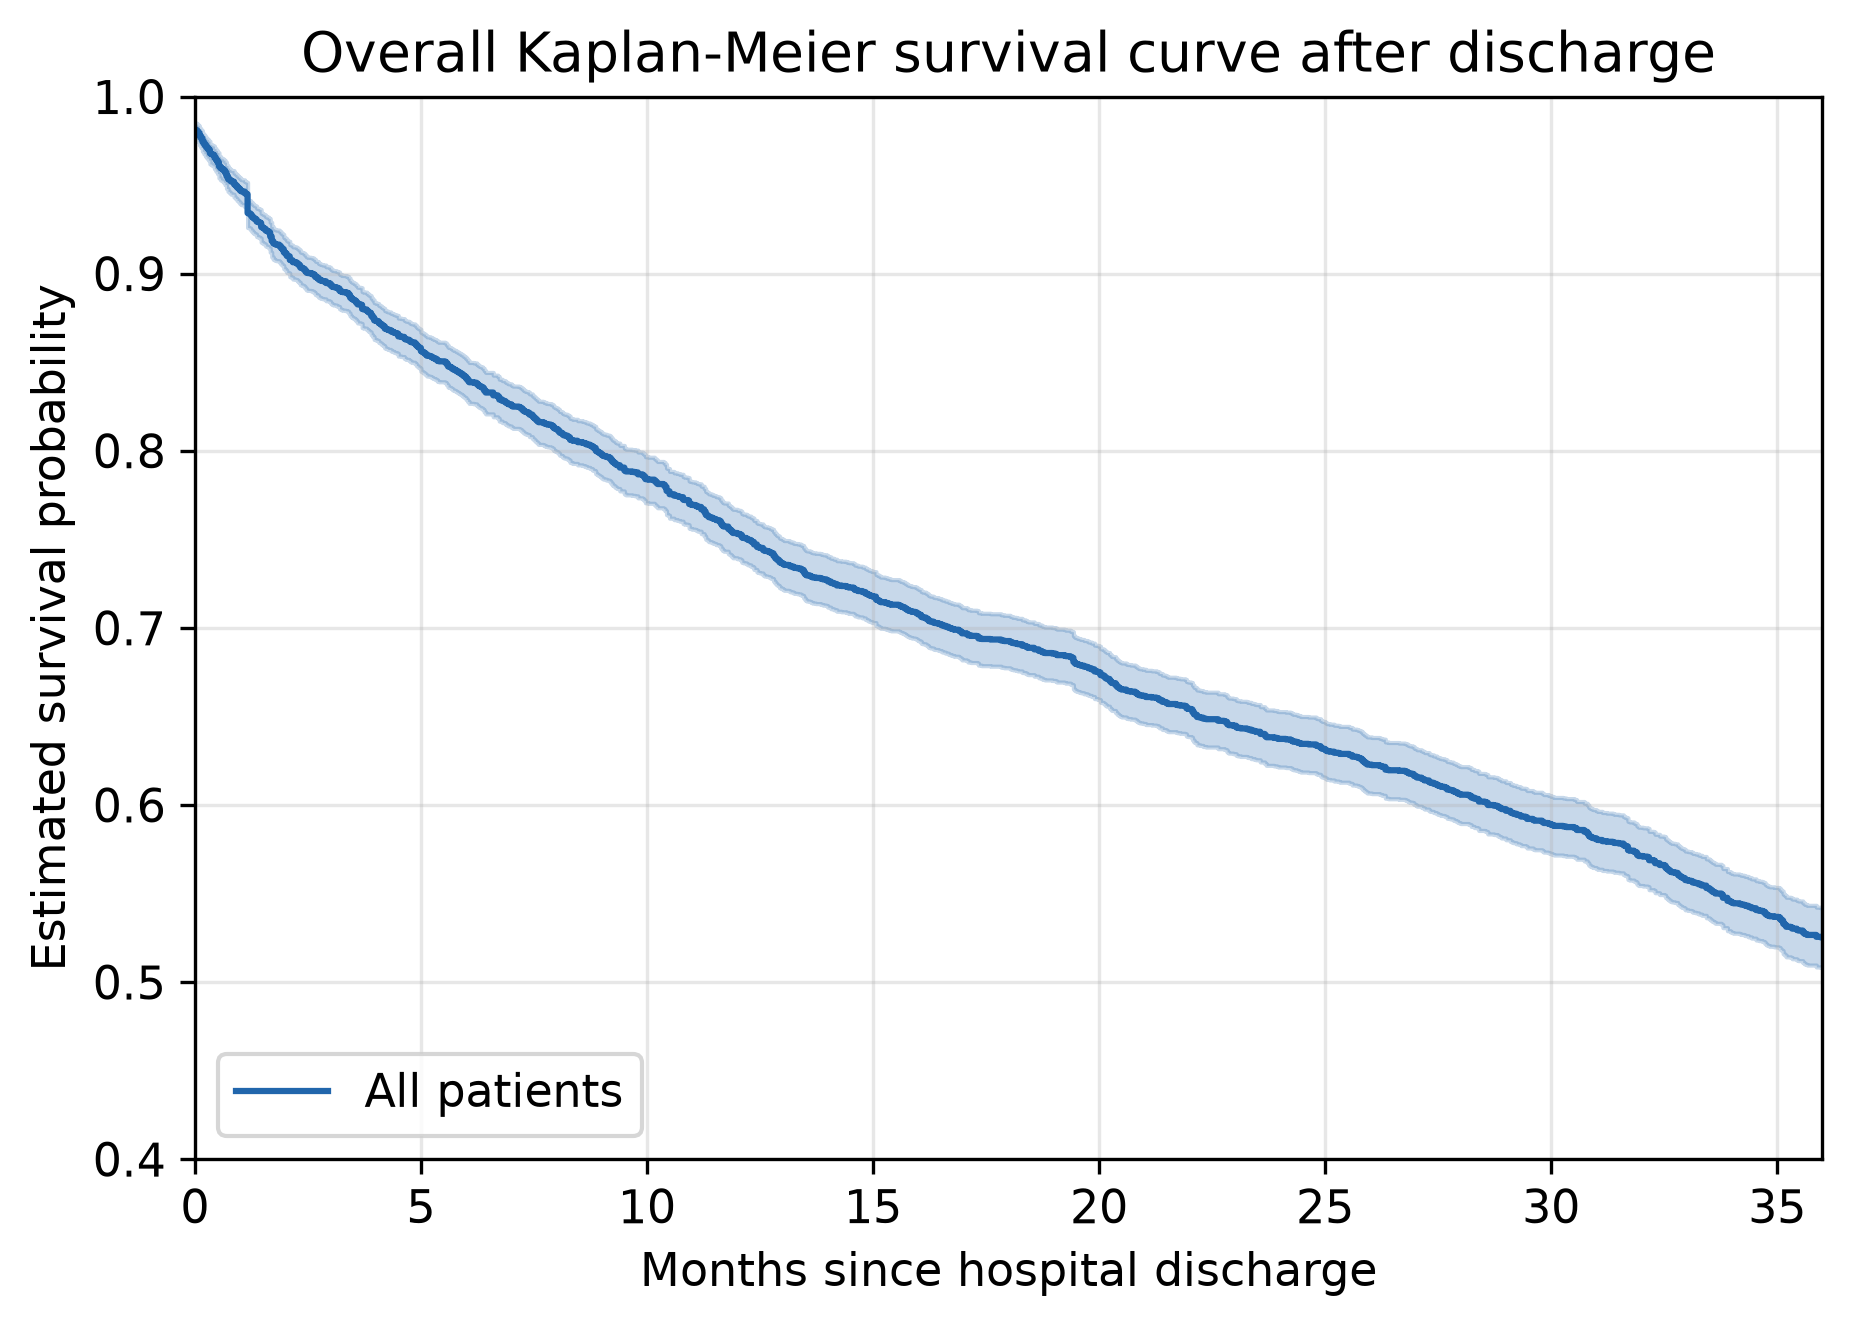
\includegraphics[width=0.72\linewidth]{fig1.png}
\end{figure}

\begin{figure}[H]
\centering
\caption{Kaplan--Meier curves stratified at the median of age (left, 76
years) and of discharge BUN (right, 28\,mg/dL), with 95\% confidence bands.}
\label{fig:km-age-bun}
\vspace{0.4em}
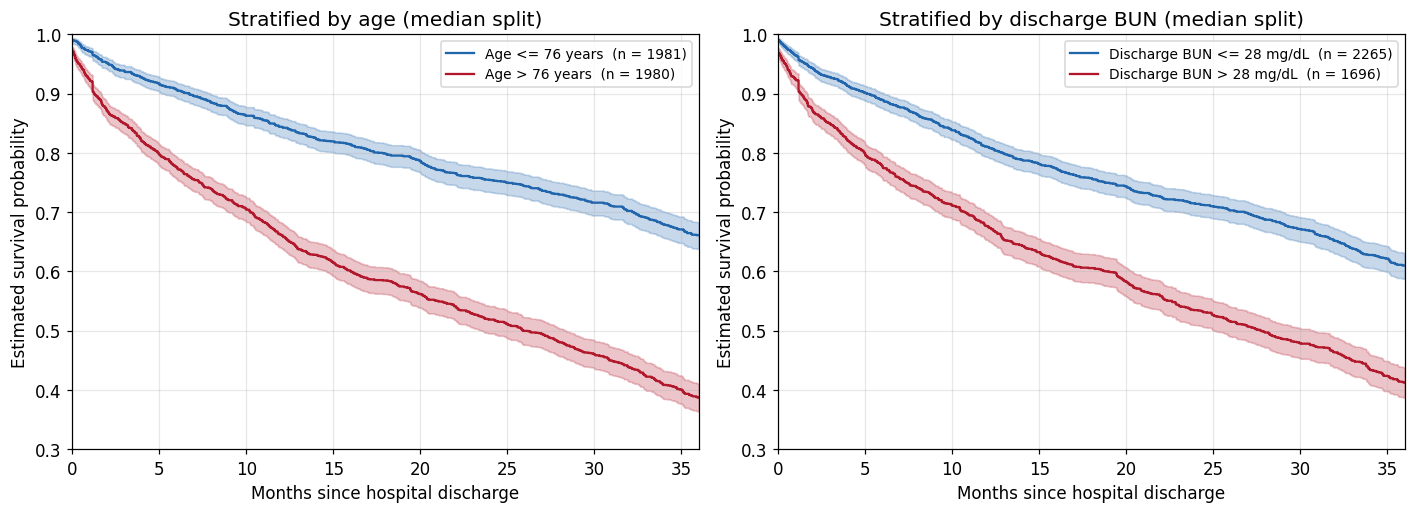
\includegraphics[width=0.98\linewidth]{fig2.png}
\end{figure}

\begin{figure}[H]
\centering
\caption{Predicted one-year survival from the PA2 Cox model and the
log-normal AFT model, sweeping age, RDW and discharge BUN in turn across the full observed
range with the remaining covariates at representative values.}
\label{fig:cox-aft}
\vspace{0.4em}
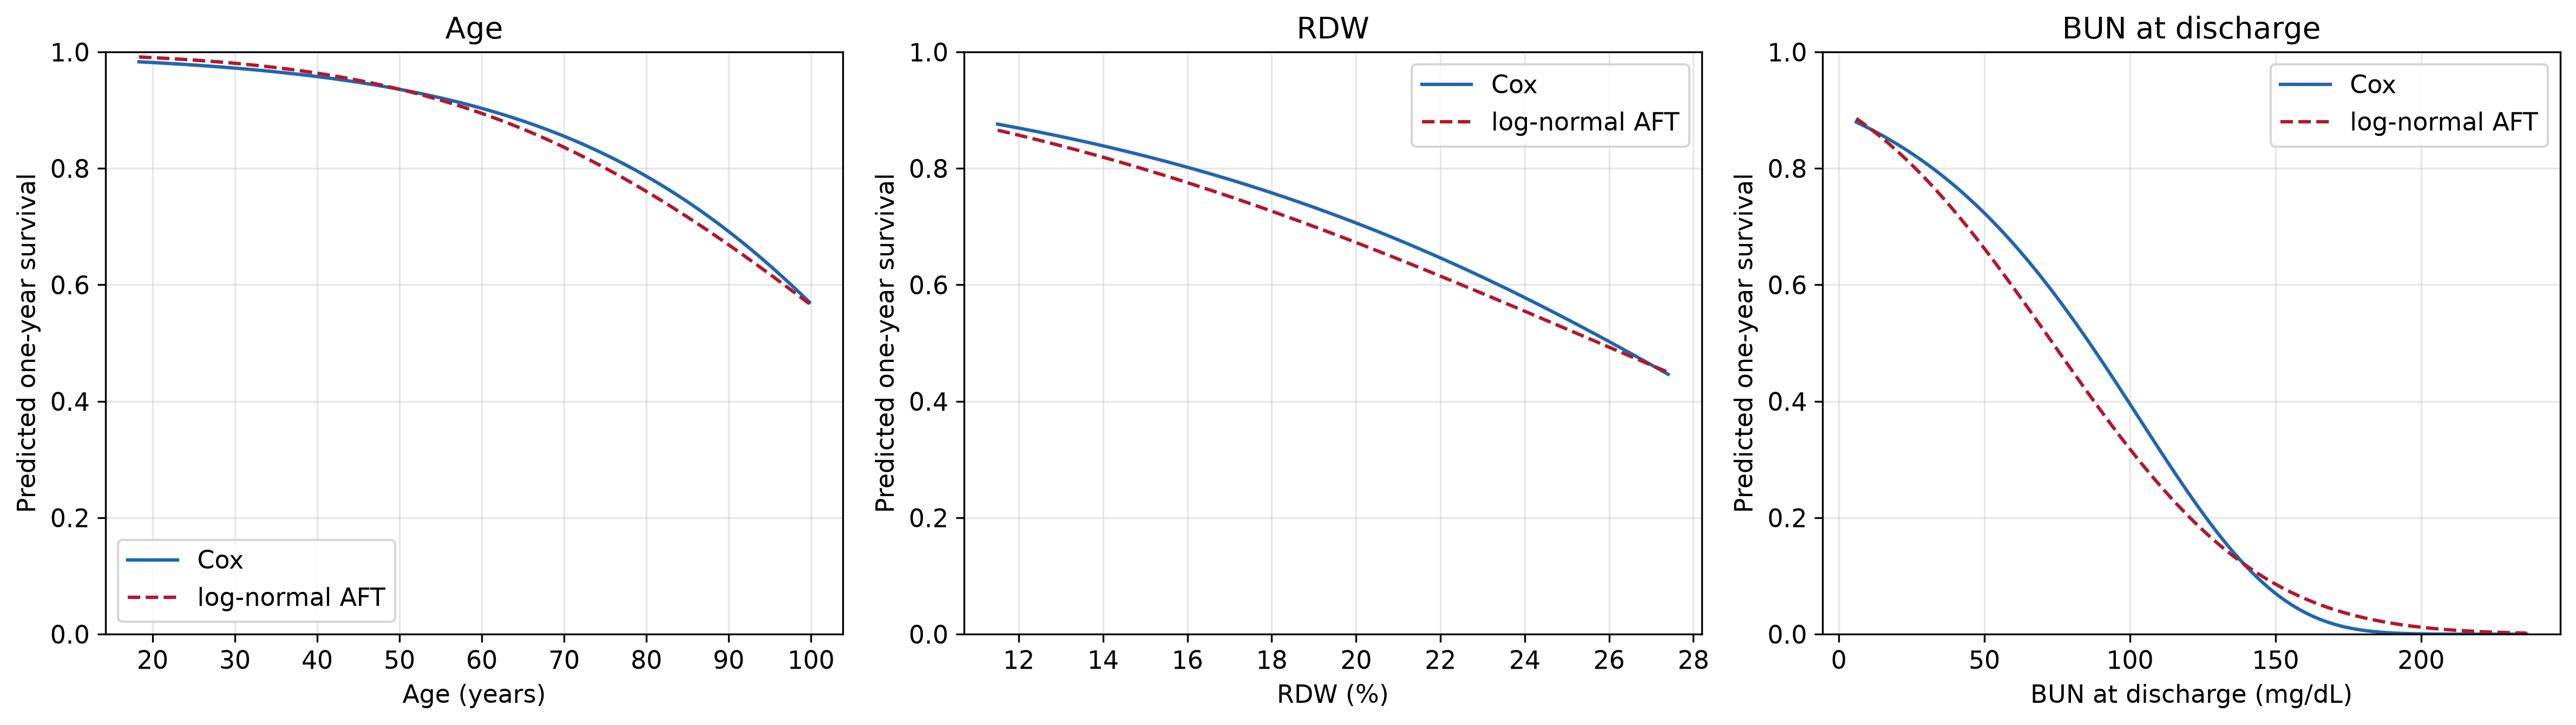
\includegraphics[width=0.98\linewidth]{fig3.png}
\end{figure}

\begin{figure}[H]
\centering
\caption{Predicted one-year survival from the Cox model fitted on the
training data, as a function of age, RDW and discharge BUN in turn. Remaining covariates are
held at their training representative values. The dotted line marks the representative
patient's predicted survival of 0.821; each curve crosses it at the covariate's median.
Grids run from the 1st to the 99th training percentile.}
\label{fig:cox-oneyear}
\vspace{0.4em}
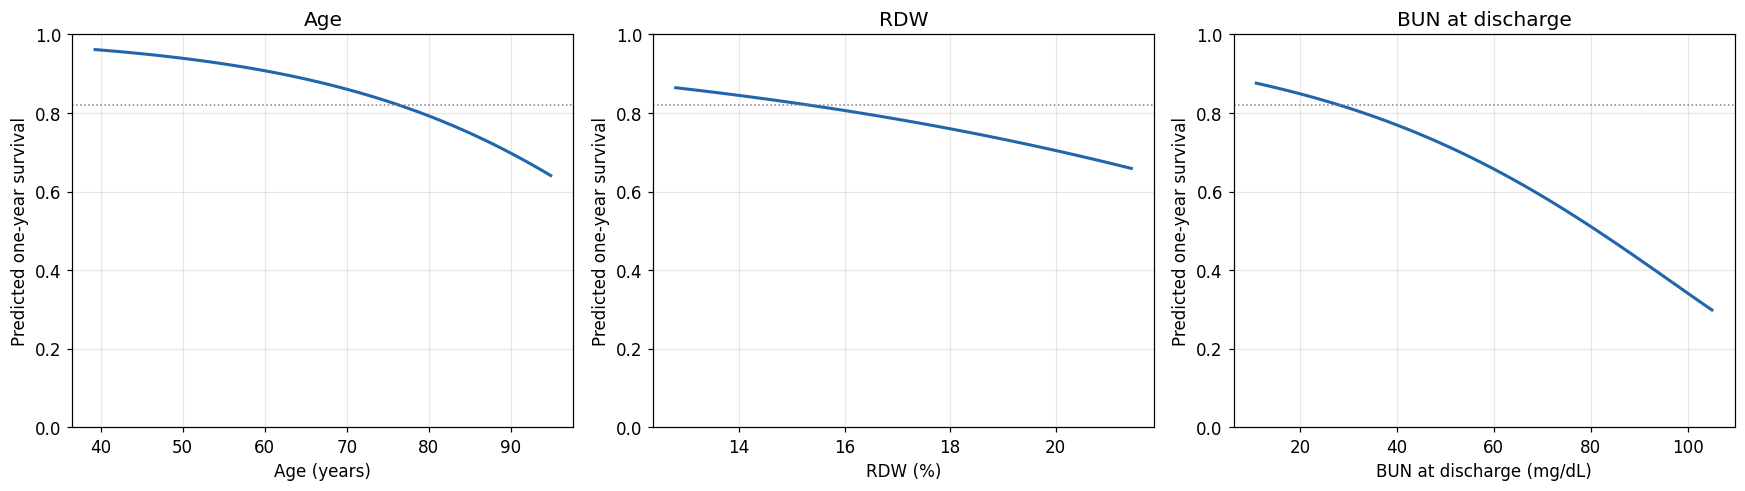
\includegraphics[width=0.98\linewidth]{fig4.png}
\end{figure}

\begin{figure}[H]
\centering
\caption{Predicted one-year survival as a function of age (top left),
RDW (top right) and discharge BUN (bottom) for the Cox model, the random survival forest,
DeepSurv and Cox-Time. All four use identical covariate grids and identical representative
values for the remaining covariates.}
\label{fig:model-curves}
\vspace{0.4em}
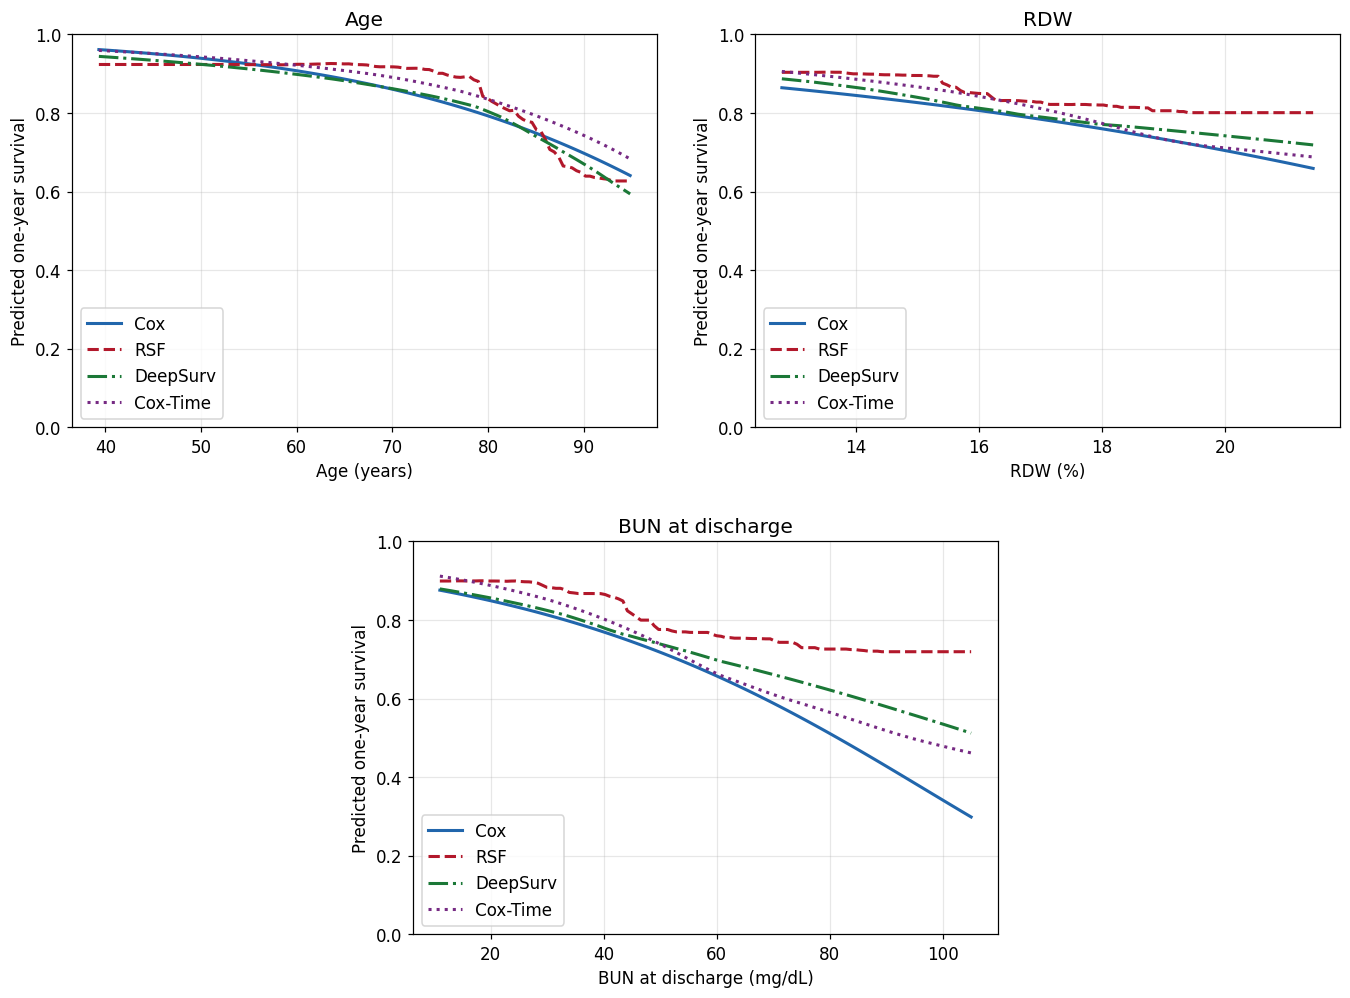
\includegraphics[width=0.90\linewidth]{fig5.png}
\end{figure}

\begin{figure}[H]
\centering
\caption{Calibration of the four models on the test set. Test patients
are divided into deciles of predicted one-year survival; each point plots mean predicted
against the Kaplan--Meier estimate of observed one-year survival in that decile, with 95\%
confidence intervals. The dotted line is the diagonal.}
\label{fig:calibration}
\vspace{0.4em}
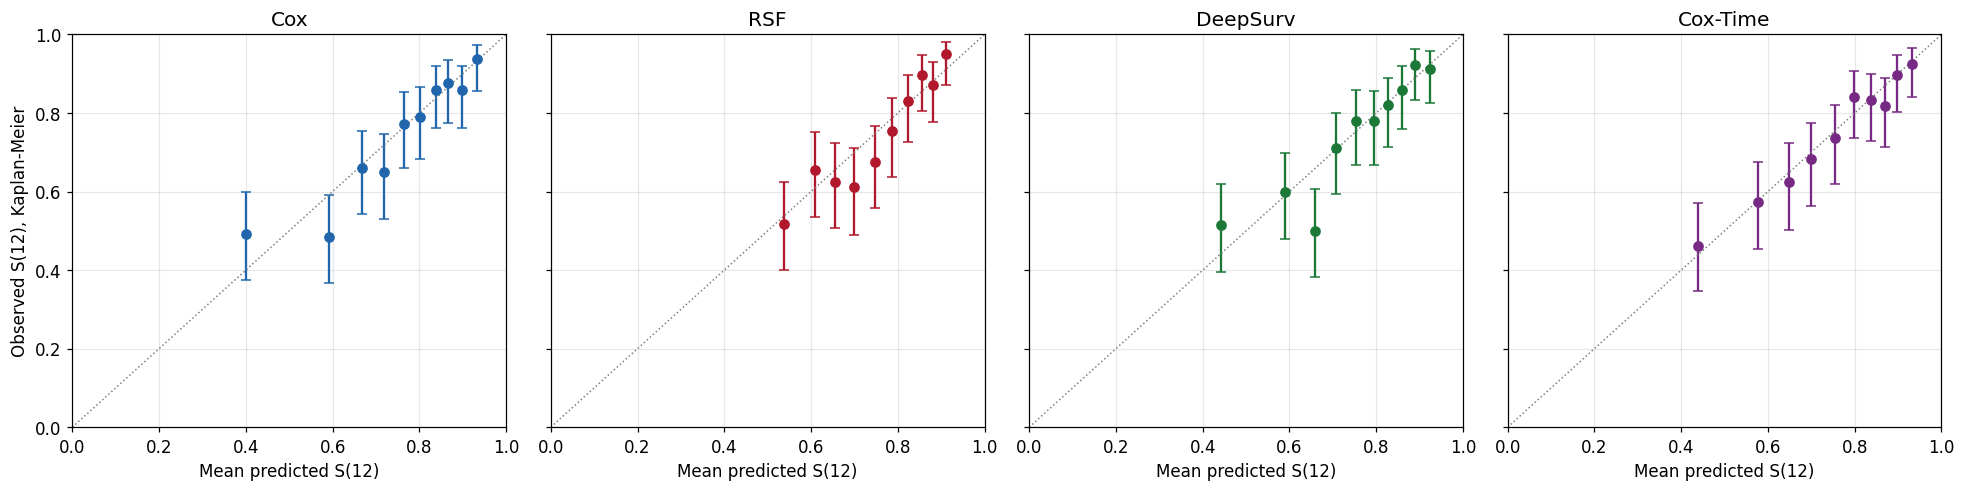
\includegraphics[width=1.0\linewidth]{fig6.png}
\end{figure}

\begin{figure}[H]
\centering
\caption{Kaplan--Meier curves for the test set split into tertiles of
predicted one-year risk, by the Cox model (left) and by the random survival forest (right),
with 95\% confidence bands.}
\label{fig:risk-tertiles}
\vspace{0.4em}
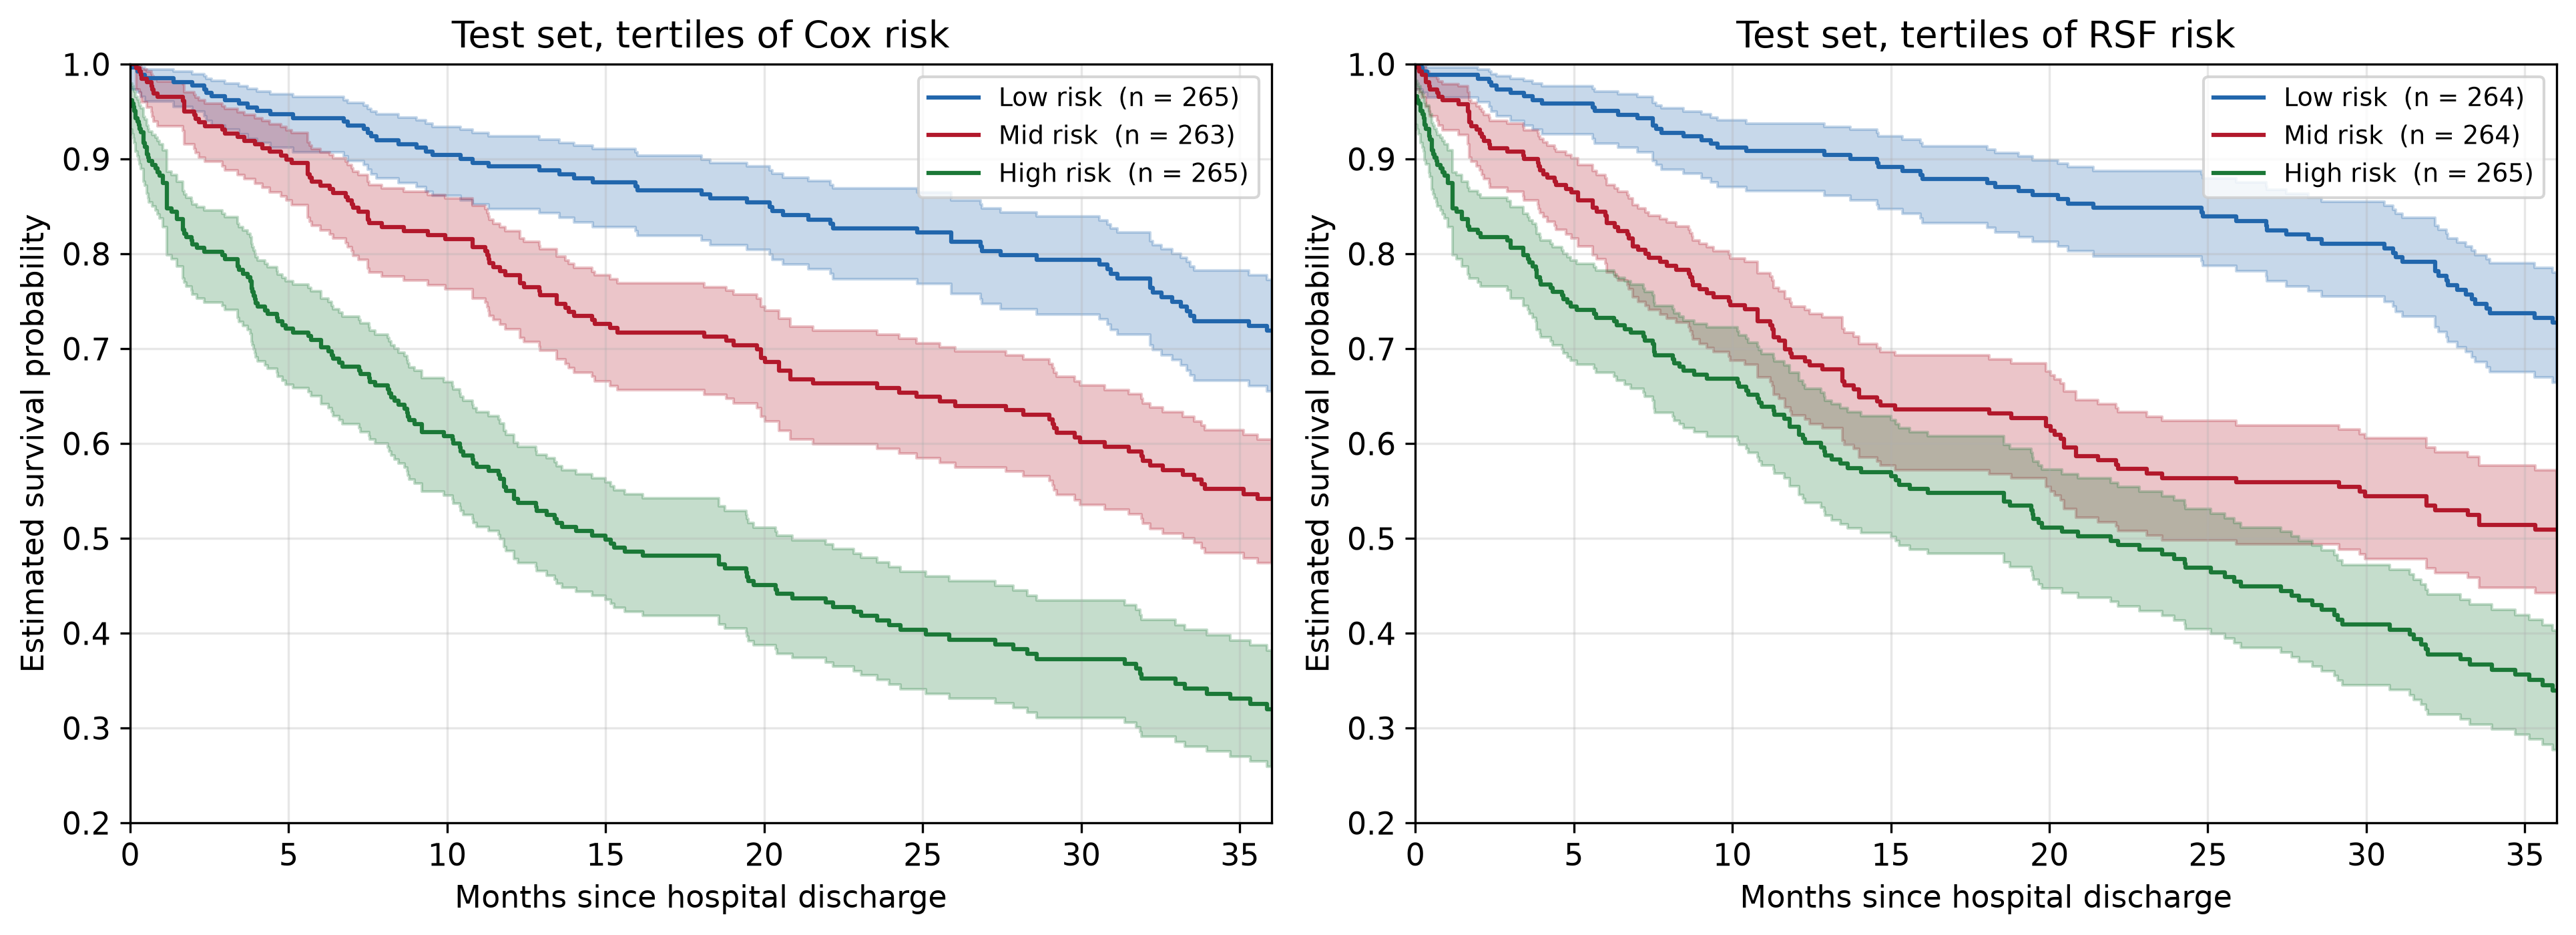
\includegraphics[width=0.98\linewidth]{fig7.png}
\end{figure}

\begin{figure}[H]
\centering
\caption{Predicted one-year survival under each interaction model,
compared with the additive Cox model (black dashed). Left: as a function of \dbun{}, with
discharge BUN at its training Q1, median and Q3. Right: as a function of discharge BUN, with
age at its training Q1, median and Q3.}
\label{fig:interactions}
\vspace{0.4em}
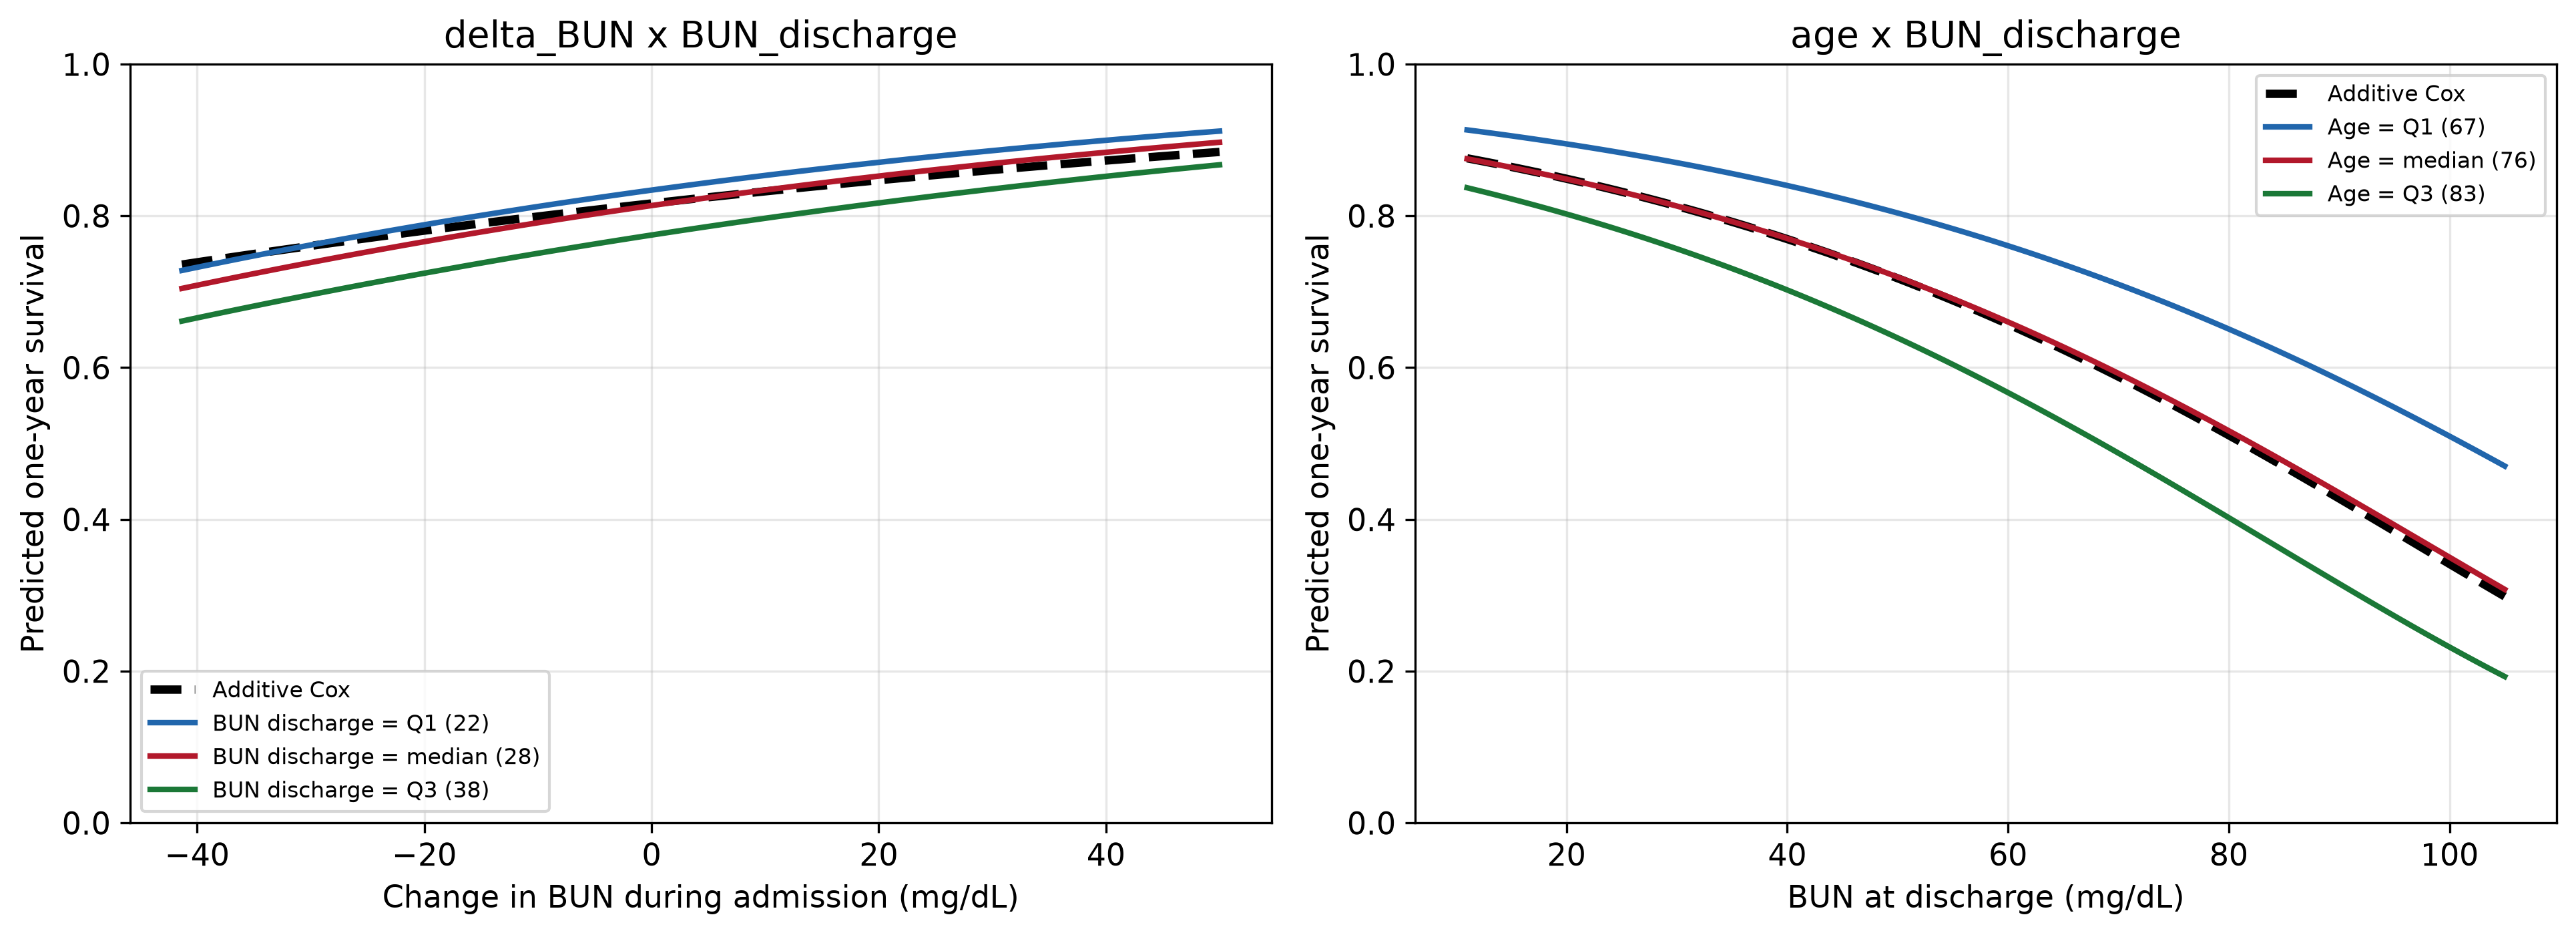
\includegraphics[width=0.98\linewidth]{fig8.png}
\end{figure}

\setcounter{figure}{0}
\renewcommand{\thefigure}{A\arabic{figure}}
\begin{figure}[H]
\centering
\caption{Scaled Schoenfeld residuals against time since discharge for
every term in the Cox model refitted on the training data, each with a lowess smoother
(red). Flat smoothers are consistent with proportional hazards. The comorbidity burden
panels fall into bands rather than a cloud because the variable enters as dummy indicators,
which is a feature of the coding and not evidence of a violation.}
\label{fig:schoenfeld}
\vspace{0.4em}
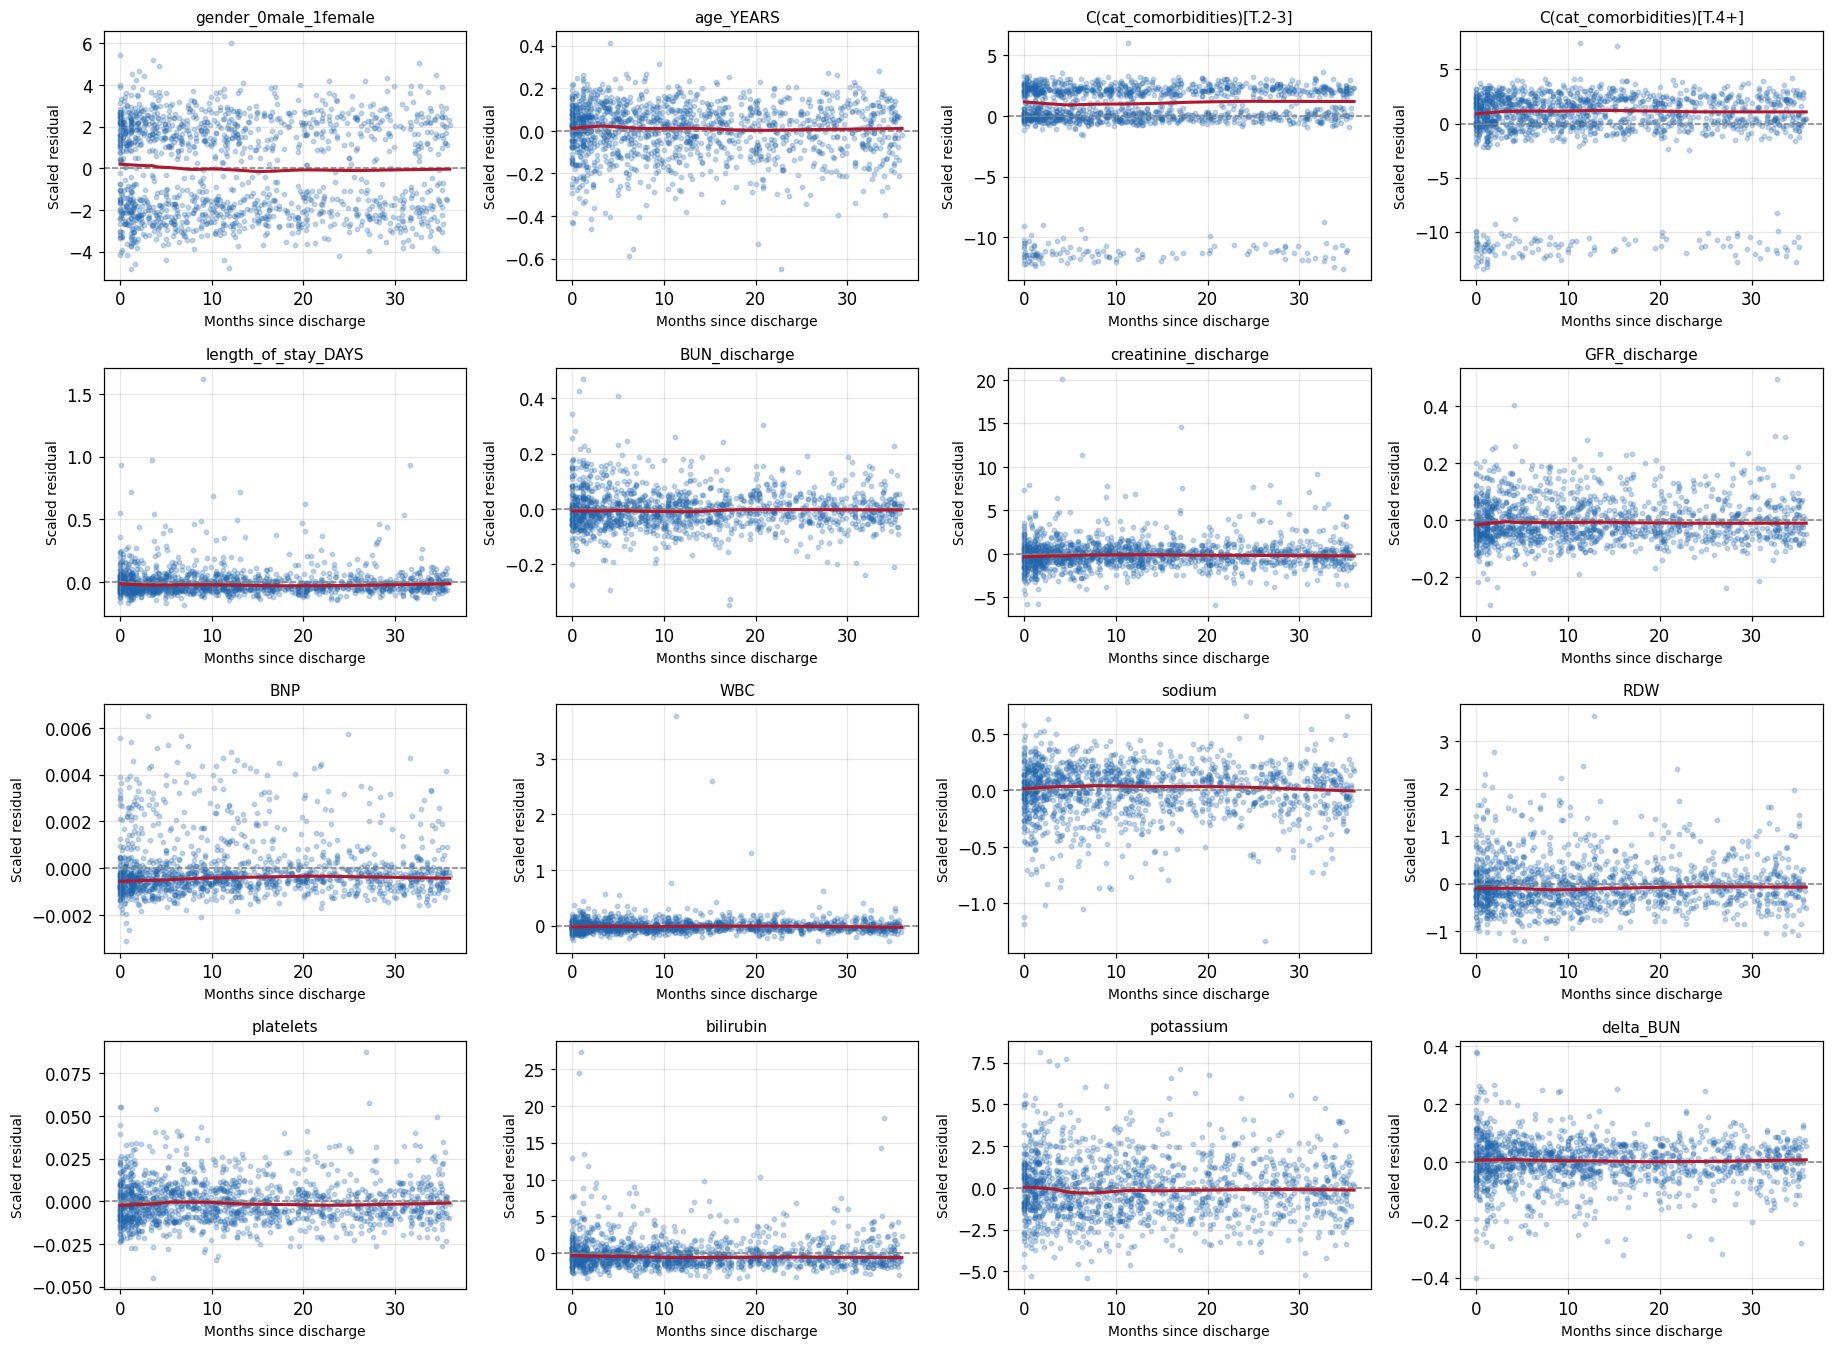
\includegraphics[width=1.0\linewidth]{figA1.png}
\end{figure}

\begin{figure}[H]
\centering
\caption{Kaplan--Meier curves stratified by sex (left) and by diabetes
(right), as examined in PA1, with 95\% confidence bands. Neither variable separates the
cohort: one-year survival is 0.770 against 0.733 by sex and 0.740 against 0.764 by diabetes.}
\label{fig:km-sex-dm}
\vspace{0.4em}
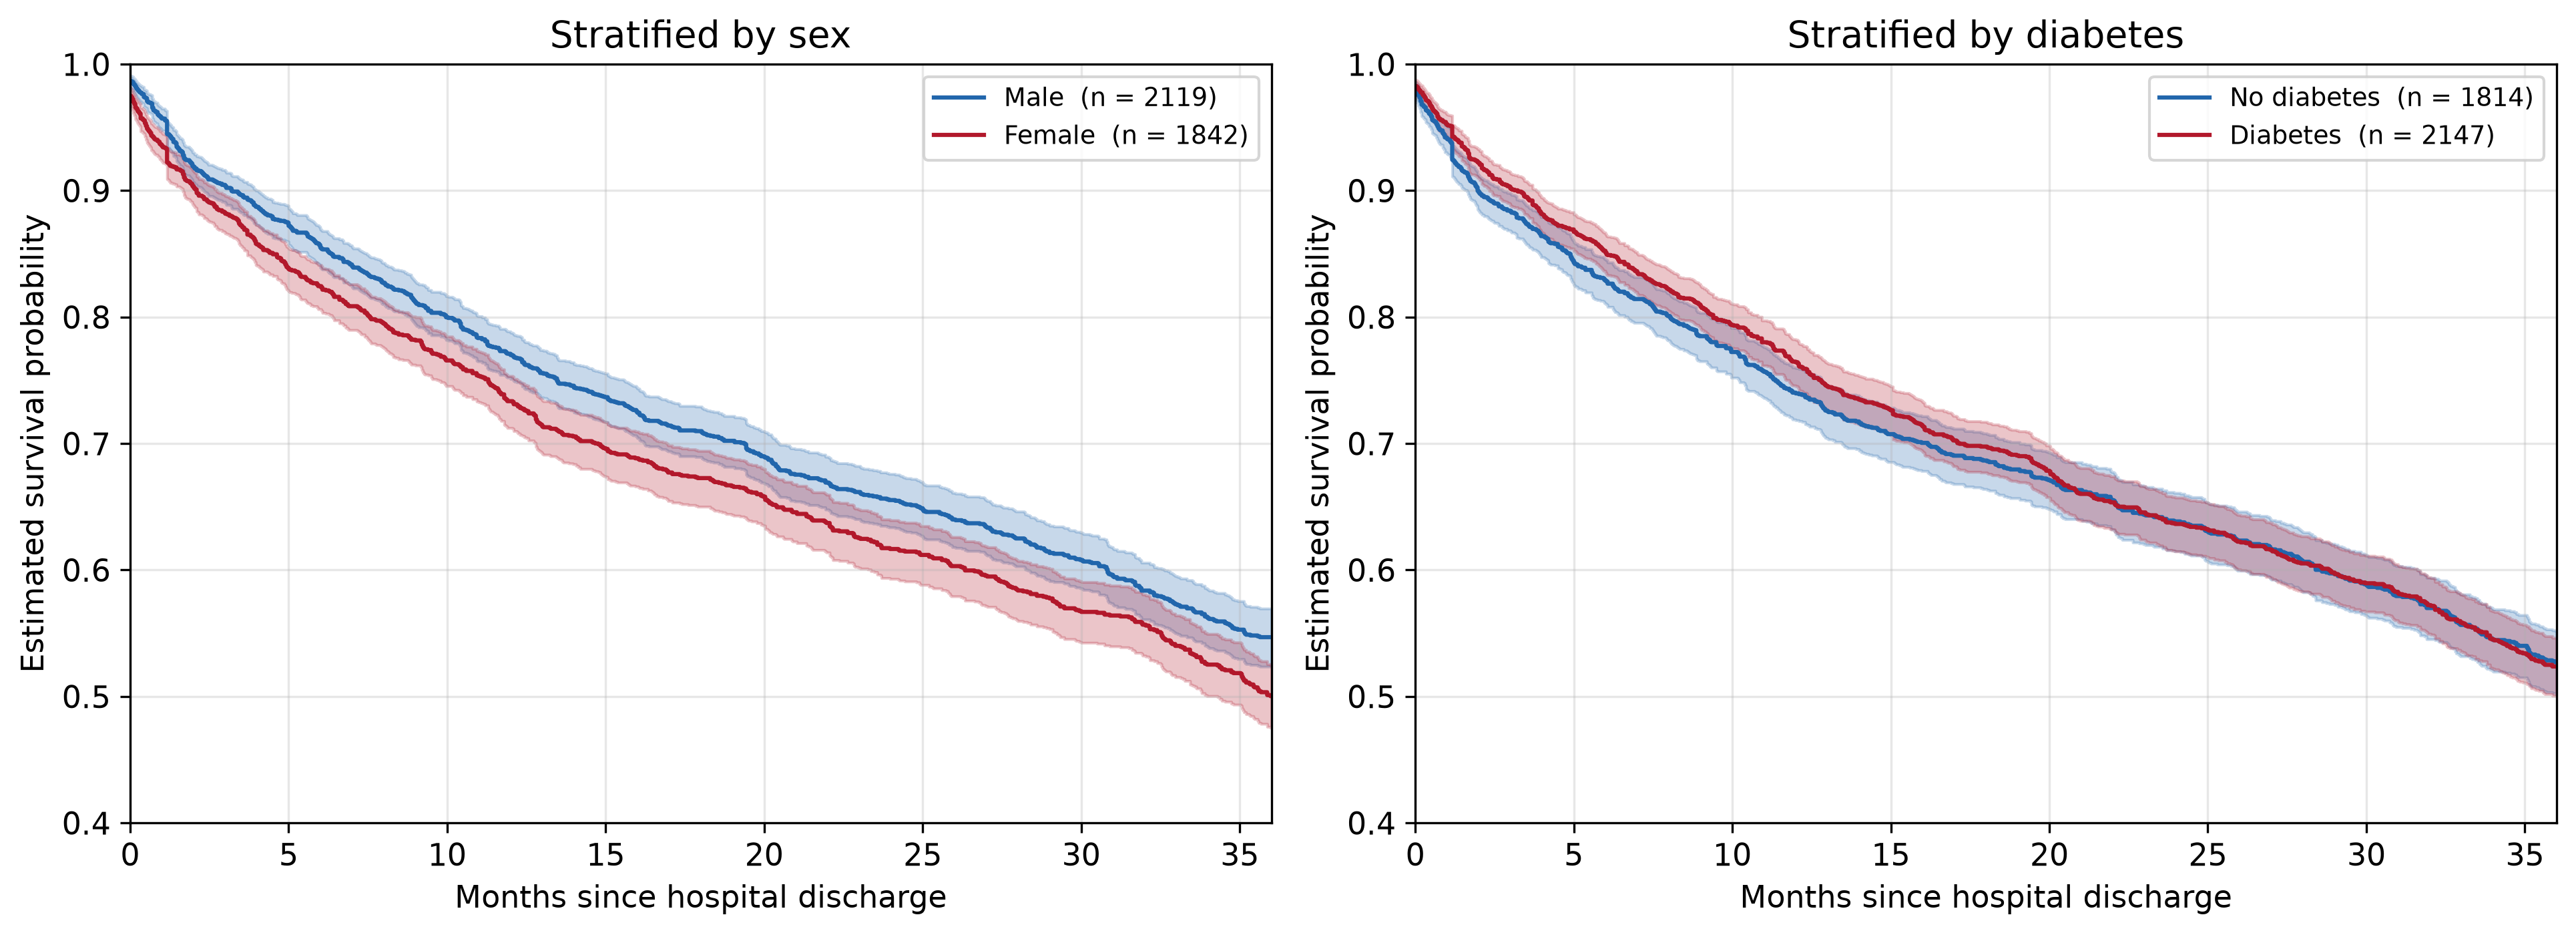
\includegraphics[width=0.98\linewidth]{figA2.png}
\end{figure}

%======================================================================
\clearpage
\section*{Tables}
\addcontentsline{toc}{section}{Tables}
\setcounter{table}{0}

\begin{table}[H]
\centering
\caption{Sample size, observed events and the composition of censoring.}
\label{tab:cohort}
\vspace{0.3em}
\small
\begin{tabular}{lcc}
\toprule
 & $n$ & \% of cohort \\
\midrule
Patients (sample size)                            & 3,961 & 100.0 \\
Observed deaths (death $=$ 1)                     & 1,679 & 42.4 \\
Censored observations (death $=$ 0)               & 2,282 & 57.6 \\
\quad of which administratively censored at 36 months & 1,473 & 37.2 \\
\quad of which lost to follow-up before 36 months     & 809   & 20.4 \\
\bottomrule
\end{tabular}
\end{table}

\begin{table}[H]
\centering
\caption{Covariate summary for all 3,961 patients. Continuous variables
are given as median [Q1, Q3] and binary variables as $n$ (\%).}
\label{tab:covariates}
\vspace{0.3em}
\small
\begin{tabular}{lcc}
\toprule
Covariate & Summary & All patients ($n = 3{,}961$) \\
\midrule
\multicolumn{3}{l}{\itshape Demographics} \\
Age (years)                          & median [Q1, Q3] & 76.18 [66.85, 83.24] \\
Female sex                           & $n$ (\%)        & 1,842 (46.5\%) \\
\addlinespace
\multicolumn{3}{l}{\itshape Comorbidities (as recorded in PA1)} \\
Diabetes                             & $n$ (\%) & 2,147 (54.2\%) \\
Hypertension                         & $n$ (\%) & 3,432 (86.6\%) \\
COPD                                 & $n$ (\%) & 405 (10.2\%) \\
Peripheral vascular disease          & $n$ (\%) & 367 (9.3\%) \\
Chronic kidney disease               & $n$ (\%) & 805 (20.3\%) \\
Ischaemic heart disease              & $n$ (\%) & 2,484 (62.7\%) \\
Atrial fibrillation                  & $n$ (\%) & 1,608 (40.6\%) \\
Valvular heart disease               & $n$ (\%) & 981 (24.8\%) \\
Pulmonary hypertension               & $n$ (\%) & 737 (18.6\%) \\
\addlinespace
\multicolumn{3}{l}{\itshape Laboratory values on admission} \\
BNP (pg/mL)                          & median [Q1, Q3] & 778.10 [734.38, 832.40] \\
BUN (mg/dL)                          & median [Q1, Q3] & 25.00 [19.00, 37.00] \\
Creatinine (mg/dL)                   & median [Q1, Q3] & 1.23 [0.95, 1.70] \\
GFR (mL/min/1.73\,m$^2$)             & median [Q1, Q3] & 49.84 [34.64, 67.64] \\
\addlinespace
\multicolumn{3}{l}{\itshape Laboratory values on discharge} \\
BUN (mg/dL)                          & median [Q1, Q3] & 28.00 [22.00, 39.00] \\
Creatinine (mg/dL)                   & median [Q1, Q3] & 1.23 [1.00, 1.56] \\
GFR (mL/min/1.73\,m$^2$)             & median [Q1, Q3] & 50.43 [34.76, 67.63] \\
\addlinespace
\multicolumn{3}{l}{\itshape Other laboratory values} \\
White blood cells (1000/$\mu$L)      & median [Q1, Q3] & 8.92 [7.00, 11.42] \\
Sodium (mEq/L)                       & median [Q1, Q3] & 138.00 [135.00, 140.00] \\
Red cell distribution width, RDW (\%)& median [Q1, Q3] & 15.30 [14.50, 16.10] \\
Platelets (1000/$\mu$L)              & median [Q1, Q3] & 225.00 [180.00, 280.30] \\
Bilirubin (mg/dL)                    & median [Q1, Q3] & 0.60 [0.50, 0.72] \\
Potassium (mEq/L)                    & median [Q1, Q3] & 4.30 [3.90, 4.60] \\
\addlinespace
\multicolumn{3}{l}{\itshape Hospitalisation} \\
Length of stay (days)                & median [Q1, Q3] & 5.13 [3.08, 8.34] \\
\bottomrule
\end{tabular}
\end{table}

\begin{table}[H]
\centering
\caption{The Cox model selected in PA2, fitted to the full dataset
($n = 3{,}961$), ordered by $p$-value. HR $=$ hazard ratio.}
\label{tab:pa2cox}
\vspace{0.3em}
\small
\begin{tabular}{lccc}
\toprule
Covariate & HR & 95\% CI & $p$ \\
\midrule
Age (years)            & 1.0438 & 1.0382 -- 1.0495 & $<$ 0.001 \\
BUN, discharge         & 1.0213 & 1.0176 -- 1.0249 & $<$ 0.001 \\
Sodium                 & 0.9728 & 0.9627 -- 0.9831 & $<$ 0.001 \\
BNP                    & 1.0002 & 1.0001 -- 1.0002 & $<$ 0.001 \\
\dbun{}                & 0.9903 & 0.9867 -- 0.9938 & $<$ 0.001 \\
RDW                    & 1.1204 & 1.0903 -- 1.1514 & $<$ 0.001 \\
Length of stay         & 1.0094 & 1.0037 -- 1.0151 & 0.001 \\
Bilirubin              & 1.1208 & 1.0068 -- 1.2477 & 0.037 \\
Potassium              & 0.9141 & 0.8397 -- 0.9951 & 0.038 \\
Platelets              & 1.0004 & 0.9999 -- 1.0009 & 0.100 \\
Creatinine, discharge  & 0.9376 & 0.8622 -- 1.0195 & 0.132 \\
Comorbidity burden 2--3& 0.8885 & 0.7431 -- 1.0624 & 0.195 \\
White blood cells      & 1.0028 & 0.9958 -- 1.0098 & 0.436 \\
Female sex             & 0.9693 & 0.8732 -- 1.0759 & 0.558 \\
GFR, discharge         & 1.0010 & 0.9975 -- 1.0045 & 0.585 \\
Comorbidity burden 4+  & 0.9882 & 0.8243 -- 1.1846 & 0.898 \\
\bottomrule
\end{tabular}
\end{table}

\begin{table}[H]
\centering
\caption{The 80/20 stratified train--test split at seed 42.}
\label{tab:split}
\vspace{0.3em}
\small
\begin{tabular}{lcccc}
\toprule
Set & $n$ & Events & Event rate & Deaths by 12 months \\
\midrule
Training & 3,168 & 1,343 & 0.424 & 748 \\
Test     & 793   & 336   & 0.424 & 199 \\
\bottomrule
\end{tabular}
\end{table}

\begin{table}[H]
\centering
\caption{Selected configuration for each model with its cross-validated
IBS over the first year (mean and standard error across the five folds). The Cox row is a
reference scored on the same folds; these scores selected the configurations and are not
performance estimates.}
\label{tab:hyper}
\vspace{0.3em}
\small
\begin{tabular}{llcc}
\toprule
Model & Selected configuration & CV IBS & SE \\
\midrule
Cox (reference) & no tuning                                        & 0.1097 & 0.0030 \\
RSF             & 500 trees, min leaf $=$ 50, max features $=$ 4   & 0.1116 & 0.0033 \\
DeepSurv        & hidden [16], dropout 0.4, lr 0.001, 119 epochs   & 0.1096 & 0.0027 \\
Cox-Time        & hidden [16], dropout 0.4, lr 0.01, 32 epochs     & 0.1105 & 0.0030 \\
\bottomrule
\end{tabular}
\end{table}

\begin{table}[H]
\centering
\caption{The selected Cox model refitted on the training data
($n = 3{,}168$, 1,343 events), with the full-data estimates of \tabref{tab:pa2cox} for comparison. Rows
are ordered by the full-data $p$-value.}
\label{tab:coxtrain}
\vspace{0.3em}
\small
\begin{tabular}{lccccc}
\toprule
Covariate & HR (train) & 95\% CI (train) & $p$ (train) & HR (full) & $p$ (full) \\
\midrule
Age (years)             & 1.0447 & 1.0384 -- 1.0511 & $<$ 0.001 & 1.0438 & $<$ 0.001 \\
BUN, discharge          & 1.0238 & 1.0197 -- 1.0279 & $<$ 0.001 & 1.0213 & $<$ 0.001 \\
RDW                     & 1.1295 & 1.0963 -- 1.1638 & $<$ 0.001 & 1.1204 & $<$ 0.001 \\
\dbun{}                 & 0.9900 & 0.9861 -- 0.9940 & $<$ 0.001 & 0.9903 & $<$ 0.001 \\
BNP                     & 1.0002 & 1.0001 -- 1.0002 & $<$ 0.001 & 1.0002 & $<$ 0.001 \\
Sodium                  & 0.9726 & 0.9611 -- 0.9843 & $<$ 0.001 & 0.9728 & $<$ 0.001 \\
Length of stay          & 1.0083 & 1.0020 -- 1.0146 & 0.010 & 1.0094 & 0.001 \\
Bilirubin               & 1.0988 & 0.9738 -- 1.2400 & 0.126 & 1.1208 & 0.037 \\
Potassium               & 0.9196 & 0.8376 -- 1.0096 & 0.078 & 0.9141 & 0.038 \\
Platelets               & 1.0005 & 0.9998 -- 1.0012 & 0.147 & 1.0004 & 0.100 \\
Creatinine, discharge   & 0.9172 & 0.8345 -- 1.0080 & 0.073 & 0.9376 & 0.132 \\
Comorbidity burden 2--3 & 0.8754 & 0.7181 -- 1.0672 & 0.188 & 0.8885 & 0.195 \\
White blood cells       & 1.0001 & 0.9918 -- 1.0085 & 0.976 & 1.0028 & 0.436 \\
Female sex              & 0.9809 & 0.8720 -- 1.1035 & 0.749 & 0.9693 & 0.558 \\
GFR, discharge          & 1.0014 & 0.9975 -- 1.0053 & 0.492 & 1.0010 & 0.585 \\
Comorbidity burden 4+   & 0.9835 & 0.8046 -- 1.2021 & 0.871 & 0.9882 & 0.898 \\
\bottomrule
\end{tabular}
\end{table}

\begin{table}[H]
\centering
\caption{Schoenfeld residual test for proportional hazards on a rank
transform of time, for the refitted model on the training data and the PA2 model on the full
data. Rows are ordered by the training $p$-value.}
\label{tab:ph}
\vspace{0.3em}
\small
\begin{tabular}{lcccc}
\toprule
Covariate & Statistic (train) & $p$ (train) & Statistic (full) & $p$ (full) \\
\midrule
Comorbidity burden 4+   & 5.366 & 0.021 & 2.700 & 0.100 \\
Comorbidity burden 2--3 & 5.060 & 0.025 & 1.388 & 0.239 \\
Bilirubin               & 4.452 & 0.035 & 2.454 & 0.117 \\
Creatinine, discharge   & 3.159 & 0.076 & 2.740 & 0.098 \\
BUN, discharge          & 2.465 & 0.116 & 4.392 & 0.036 \\
Length of stay          & 2.217 & 0.137 & 3.911 & 0.048 \\
\dbun{}                 & 2.141 & 0.143 & 0.625 & 0.429 \\
Female sex              & 1.709 & 0.191 & 1.269 & 0.260 \\
GFR, discharge          & 1.031 & 0.310 & 0.828 & 0.363 \\
Potassium               & 0.963 & 0.326 & 0.601 & 0.438 \\
Age (years)             & 0.452 & 0.501 & 1.064 & 0.302 \\
Sodium                  & 0.289 & 0.591 & 1.643 & 0.200 \\
White blood cells       & 0.237 & 0.627 & 0.121 & 0.728 \\
BNP                     & 0.208 & 0.649 & 0.087 & 0.768 \\
Platelets               & 0.004 & 0.951 & 0.225 & 0.636 \\
RDW                     & 0.000 & 0.991 & 0.025 & 0.875 \\
\bottomrule
\end{tabular}
\end{table}

\begin{table}[H]
\centering
\caption{Predicted one-year survival at the ends of each plotted grid and
across each covariate's interquartile range, from the Cox model fitted on the training data.}
\label{tab:coxpred}
\vspace{0.3em}
\footnotesize
\begin{tabular}{lccccc}
\toprule
Covariate & Grid (1st--99th pct) & $S$ at low & $S$ at high & Drop over grid & Drop over IQR \\
\midrule
Age (years)             & 39.3 -- 94.8 & 0.962 & 0.641 & 0.321 & 0.110 \\
RDW (\%)                & 12.8 -- 21.4 & 0.864 & 0.659 & 0.205 & 0.034 \\
BUN, discharge (mg/dL)  & 11 -- 105    & 0.876 & 0.298 & 0.577 & 0.064 \\
\bottomrule
\end{tabular}
\end{table}

\begin{table}[H]
\centering
\caption{Predicted one-year survival at the ends of each plotted grid and
across each covariate's interquartile range, for all four models. The Cox rows reproduce
\tabref{tab:coxpred} exactly, confirming that all four are evaluated on the same grids and the same
representative patient.}
\label{tab:modelcurves}
\vspace{0.3em}
\footnotesize
\begin{tabular}{llcccc}
\toprule
Covariate & Model & $S$ at low & $S$ at high & Drop over grid & Drop over IQR \\
\midrule
Age (years) & Cox      & 0.962 & 0.641 & 0.321 & 0.110 \\
            & RSF      & 0.924 & 0.627 & 0.297 & 0.118 \\
            & DeepSurv & 0.945 & 0.584 & 0.361 & 0.105 \\
            & Cox-Time & 0.946 & 0.633 & 0.313 & 0.114 \\
\addlinespace
RDW (\%)    & Cox      & 0.864 & 0.659 & 0.205 & 0.034 \\
            & RSF      & 0.904 & 0.801 & 0.103 & 0.057 \\
            & DeepSurv & 0.891 & 0.709 & 0.183 & 0.044 \\
            & Cox-Time & 0.885 & 0.677 & 0.208 & 0.043 \\
\addlinespace
BUN, discharge & Cox      & 0.876 & 0.298 & 0.577 & 0.064 \\
               & RSF      & 0.899 & 0.719 & 0.180 & 0.032 \\
               & DeepSurv & 0.885 & 0.465 & 0.420 & 0.061 \\
               & Cox-Time & 0.898 & 0.389 & 0.509 & 0.078 \\
\bottomrule
\end{tabular}
\end{table}

\setcounter{table}{10}  % 10 was used inline in Section 6.4
\begin{table}[H]
\centering
\caption{Agreement between the four models on individual test-set risk. Panel (a) gives the
Spearman rank correlation between the predicted one-year risks; panel (b) the overlap between
the top-risk quintiles of each pair, 159 test patients per model.}
\label{tab:risk}
\vspace{0.3em}
\small
{\itshape (a) Spearman rank correlation}\\[0.3em]
\begin{tabular}{lcccc}
\toprule
 & Cox & RSF & DeepSurv & Cox-Time \\
\midrule
Cox      & 1.000 & 0.884 & 0.976 & 0.976 \\
RSF      & 0.884 & 1.000 & 0.911 & 0.908 \\
DeepSurv & 0.976 & 0.911 & 1.000 & 0.980 \\
Cox-Time & 0.976 & 0.908 & 0.980 & 1.000 \\
\bottomrule
\end{tabular}

\vspace{1em}
{\itshape (b) Overlap of the top-risk quintiles}\\[0.3em]
\begin{tabular}{llccc}
\toprule
Model A & Model B & Shared of 159 & Shared \% & Jaccard \\
\midrule
Cox      & RSF      & 113 & 71.1 & 0.551 \\
Cox      & DeepSurv & 141 & 88.7 & 0.797 \\
Cox      & Cox-Time & 140 & 88.1 & 0.787 \\
RSF      & DeepSurv & 124 & 78.0 & 0.639 \\
RSF      & Cox-Time & 117 & 73.6 & 0.582 \\
DeepSurv & Cox-Time & 138 & 86.8 & 0.767 \\
\bottomrule
\end{tabular}
\end{table}

\begin{table}[H]
\centering
\caption{Test-set discrimination and prediction error within subgroups
defined by the training medians of discharge BUN (28\,mg/dL) and age (76 years). $n$ is the
number of test patients, ``deaths'' the number dying within 12 months.}
\label{tab:subgroup}
\vspace{0.3em}
\small
\begin{tabular}{lllcccc}
\toprule
Subgroup & Measure & $n$ (deaths) & Cox & RSF & DeepSurv & Cox-Time \\
\midrule
BUN $\le$ 28 mg/dL & Uno's C & 430 (81) & 0.7140 & 0.6946 & 0.7018 & 0.7079 \\
                   & IBS     & 430 (81) & 0.0901 & 0.0933 & 0.0910 & 0.0899 \\
\addlinespace
BUN $>$ 28 mg/dL   & Uno's C & 363 (118) & 0.6361 & 0.6173 & 0.6346 & 0.6349 \\
                   & IBS     & 363 (118) & 0.1446 & 0.1449 & 0.1441 & 0.1431 \\
\addlinespace
Age $\le$ 76 years & Uno's C & 406 (62) & 0.6663 & 0.7010 & 0.6785 & 0.6815 \\
                   & IBS     & 406 (62) & 0.0787 & 0.0783 & 0.0786 & 0.0784 \\
\addlinespace
Age $>$ 76 years   & Uno's C & 387 (137) & 0.6172 & 0.5800 & 0.6085 & 0.6203 \\
                   & IBS     & 387 (137) & 0.1532 & 0.1574 & 0.1538 & 0.1519 \\
\bottomrule
\end{tabular}
\end{table}

\begin{table}[H]
\centering
\caption{Likelihood-ratio and Wald tests for the two pre-specified
interactions, each added as a single term to the refitted Cox model and fitted on the
training data. The likelihood-ratio statistic has 1 degree of freedom; the
Bonferroni-corrected threshold for two pre-specified tests is 0.025.}
\label{tab:interactions}
\vspace{0.3em}
\small
\begin{tabular}{lccccc}
\toprule
Interaction term & HR & 95\% CI & Wald $p$ & LR statistic & LR $p$ \\
\midrule
BUN, discharge $\times$ \dbun{} & 1.0001 & 1.0000 -- 1.0002 & 0.012 & 5.854 & 0.016 \\
Age $\times$ BUN, discharge     & 1.0001 & 0.9998 -- 1.0003 & 0.592 & 0.288 & 0.592 \\
\bottomrule
\end{tabular}
\end{table}

\begin{table}[H]
\centering
\caption{Predictive performance of the additive Cox model and each
interaction model: test-set Uno's C at $\tau = 12$ months, test-set IBS over the first year,
and cross-validated IBS on the five training folds (fold-to-fold standard error 0.0030
throughout).}
\label{tab:interperf}
\vspace{0.3em}
\small
\begin{tabular}{lccc}
\toprule
Model & Uno's C (test) & IBS (test) & CV IBS (train) \\
\midrule
Cox (additive)                          & 0.6959 & 0.1150 & 0.1097 \\
$+$ BUN, discharge $\times$ \dbun{}     & 0.6933 & 0.1152 & 0.1094 \\
$+$ Age $\times$ BUN, discharge         & 0.6955 & 0.1151 & 0.1097 \\
\bottomrule
\end{tabular}
\end{table}

\end{document}
